\documentclass[10pt,xcolor={dvipsnames}]{beamer}
\usetheme{CambridgeUS}

\usepackage[utf8]{inputenc}
\usepackage[english]{babel}
\usepackage{amsmath}
\usepackage{amsfonts}
\usepackage{amssymb}

%\usepackage[svgnames]{xcolor}

\usepackage{listings}

\usepackage{tikz} % for painting, heheheh
\usepackage{pgfplots}
\usepackage{pgfplotstable}
\usetikzlibrary{arrows,shadows,patterns, external, decorations.text,positioning, shapes}

\usepackage[absolute,overlay,showboxes]{textpos}


\author[Inti Gonzalez-Herrera]{Inti Gonzalez Herrera\\[0.5cm]{\scriptsize PhD's thesis  \\[.3cm] \textit{Supervised by}: Olivier Barais and Johann Bourcier\newline
		\textit{Jury}: Isabelle Puaut, Vivien Qu\'ema, Gilles Muller, Ga\"el Thomas, Laurent R\'eveill\`ere}}
\title[{\tiny Supporting resource-awareness in MRTEs}]{Supporting resource-awareness in managed runtime environments}
\subtitle{}
%\logo{
\includegraphics[scale=0.4]{../rennes1.pdf}}
\institute[]{Diverse -- IRISA/University of Rennes 1}
\date{\today}
\titlegraphic{\includegraphics[scale=0.5]{../diverse.png}}
%\subject{}
%\setbeamercovered{transparent}
\setbeamertemplate{navigation symbols}{}

%\usefonttheme{serif}
%\usecolortheme{lily}

\addto\captionsenglish{%
	\renewcommand{\figurename}{\scriptsize Fig.}%
}

\begin{document}
	
	% DONE - 1
	\begin{frame}
		\titlepage
	\end{frame}
	
	\section[Context]{Context}
	
	\subsection[Motivation]{Motivation}
	
	% DONE - 5
	\begin{frame}{Developers embrace managed runtime environments}
		%\textbf{Programming language popularity rating~\footnote{TIOBE Index as for Dec 2015. Just as a reference for the motivation}}:
		\begin{figure}
			\centering
			
\includegraphics[scale=0.4]{fig/languages.png}
		\end{figure}
		\begin{columns}
			\column{0.6\textwidth}
			\begin{block}{Managed runtime environments (MRTEs) \underline{boost productivity}}
				\begin{footnotesize}
					\begin{itemize}
						\item Portability of Applications
						\item Dynamic Code Loading (supporting the hypothesis of open world)
						\item Automatic Memory Management (usually with a Garbage Collector)
						\item Improved Error Handling
					\end{itemize}
				\end{footnotesize}
			\end{block}
			\column{0.25\textwidth}
			\begin{exampleblock}{MRTEs}
				\begin{figure}
					
\includegraphics[scale=0.0018]{fig/jvm.jpeg}
				\end{figure}
				\vspace{-.5cm}
				\begin{figure}
					
\includegraphics[scale=0.07]{fig/python.jpg}
				\end{figure}
				\vspace{-.5cm}
				\begin{figure}
					
\includegraphics[scale=0.17]{fig/dotnet.png}
				\end{figure}
			\end{exampleblock}
		\end{columns}
%		\begin{footnotesize}
%			\begin{itemize}
%				\item Java (20.97\%) \hfill 
\includegraphics[scale=0.0006]{fig/jvm.jpeg}
%				\item Python (4.42\%) \hfill 
\includegraphics[scale=0.03]{fig/python.jpg}
%				\item C\# (4.11\%) \hfill 
\includegraphics[scale=0.06]{fig/dotnet.png}
%				\item Visual Basic .Net (2.39\%) \hfill 
\includegraphics[scale=0.06]{fig/dotnet.png}
%			\end{itemize}
%		\end{footnotesize}
%		\vspace{0.2cm}
		%{\centering \color{red} \\}
		%\vspace{0.5cm}
		%\centering{\color{red}  But developers have limited control on how resources are used}
	\end{frame}
	
	% DONE - 2
	\begin{frame}{High usability vs Limited Control}
			\begin{columns}<1->
				\column{0.2\textwidth}
				\begin{scriptsize}
					\begin{block}{Focus on Ideas}
						\begin{itemize}
							\item Use high-level abstractions
							\item Forget about details such as resources
						\end{itemize}
					\end{block}
				\end{scriptsize}
				\column{0.75\textwidth}
					\begin{figure}
						\centering
						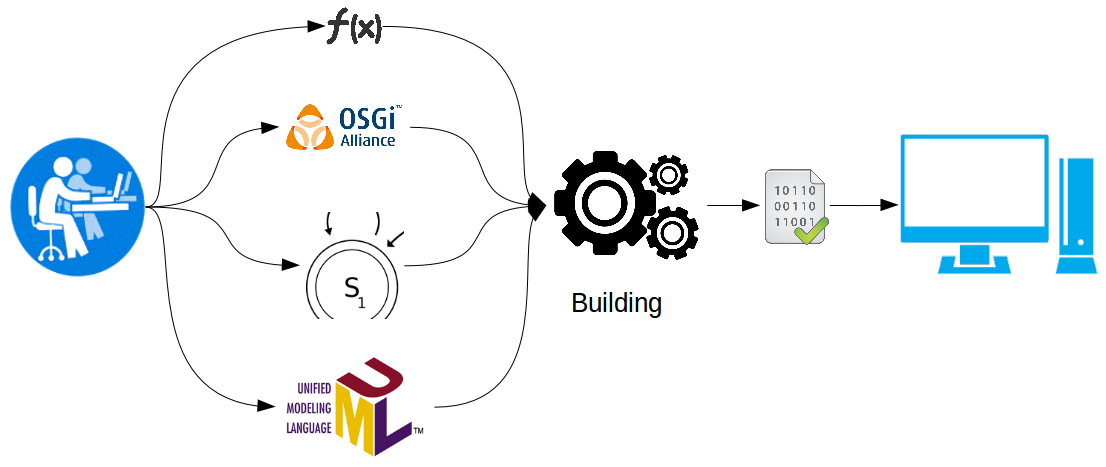
\includegraphics[scale=0.3]{fig/high-level.png}
					\end{figure}
			\end{columns}
	%		\vspace{0.2cm}
			\begin{columns}<2->
				\column{0.3\textwidth}
					\begin{figure}
						\centering
						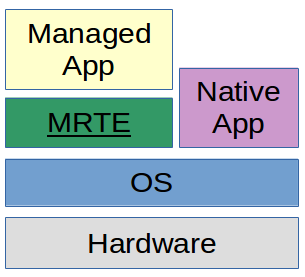
\includegraphics[scale=0.3]{fig/software-stack.png}
					\end{figure}
				  
				\column{0.65\textwidth}
				\begin{scriptsize}
					\begin{alertblock}{In the ``software stack'' we trust}
						\begin{itemize}
							\item OSs abstract the hardware
							\item OSs multiplex resource
							\item Runtimes offer additional guarantees
						\end{itemize}
					\end{alertblock}
				\end{scriptsize}
			\end{columns}
		\vspace{0.2cm}
		\uncover<2->{
		\centering{%
			\textbf{\Large \color{red} It \underline{usually} works!!!}
		}%
		}
	\end{frame}
	
	% Real Example in a new slide
	
	% DONE - 3
	\begin{frame}{But developers need control}
		\begin{footnotesize}
		\vspace{-.2cm}
		\begin{columns}
			\column{0.43\textwidth}
			\begin{exampleblock} {Developers often need support for fined-grain resource management}
				
					\begin{enumerate}[1]
						\item Developing middleware and Component Frameworks
						\item Multi-tenant cloud systems
						\item Smartphones and Embedded systems
					\end{enumerate}
			\end{exampleblock}
			\vspace{-.2cm}
			\begin{block} {A ``traditional'' \textbf{software stack} can be a burden in these cases}
				\begin{footnotesize}
					\begin{enumerate}[1]
						\item Generic APIs might hinder performance
						\item \textit{Safe} APIs prevent collecting information and managing resources
					\end{enumerate}
				\end{footnotesize}
			\end{block}
			\column{0.55\textwidth}
			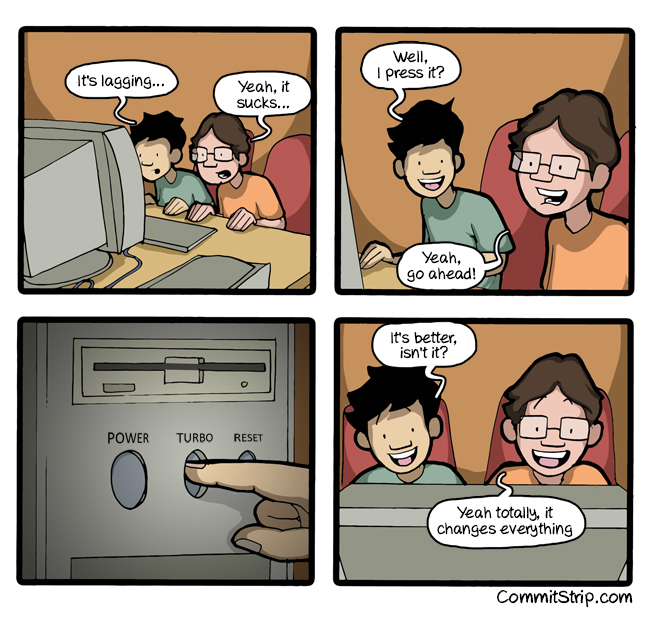
\includegraphics[scale=0.29]{fig/need-for-speed.jpg}
		\end{columns}
		\vspace{-.2cm}
		\begin{alertblock}{Consequences? }
			Suboptimal solutions 
			\begin{center}
				{\color{red} More control is needed!!!}
			\end{center}
		\end{alertblock}
		\end{footnotesize}
	\end{frame}
	
	\subsection[Problem]{Problem}
	
	% DONE - 4
	\begin{frame}{The populous land of resource-aware applications}
		\begin{block}{Resource-aware applications}
			\begin{itemize}
				\item \textbf{{Observe}}
				\begin{itemize}
					\item how \underline{different parts} of applications \underline{consume resource}?
					\item how much resources are available?
				\end{itemize}
				\item \textbf{{Manage}} the resource available
				\begin{itemize}
					\item allocating and deallocating resource as needed
				\end{itemize}
				\item \textbf{{Modify their behavior}}
				\begin{itemize}
					\item to improve performance
					\item to avoid critical failures
				\end{itemize}
			\end{itemize}
		\end{block}
		
		\begin{alertblock}{Resource-aware programming \underline{requires runtime support}}
			We focus on \underline{supporting resource-aware programming} by \underline{providing}:
			\begin{enumerate}
				\item Resource Consumption Monitoring
				\item Resource Reservation
			\end{enumerate}
		\end{alertblock}
	\end{frame}
	
	\begin{frame}{Problems}
		\vspace{-.3cm} 
		\begin{footnotesize}
			\begin{alertblock}{Mismatch between the concepts used by developers and how tools present information}
				Developers define new abstractions to deal with specific domains, but development tools (e.g., profilers and debuggers) know nothing about such abstractions. \\
				\begin{center}
					\textcolor{red}{\large We need \underline{domain-specific} development \underline{tools}}
				\end{center}
			\end{alertblock}
		\end{footnotesize}
		\begin{figure}
			\centering
			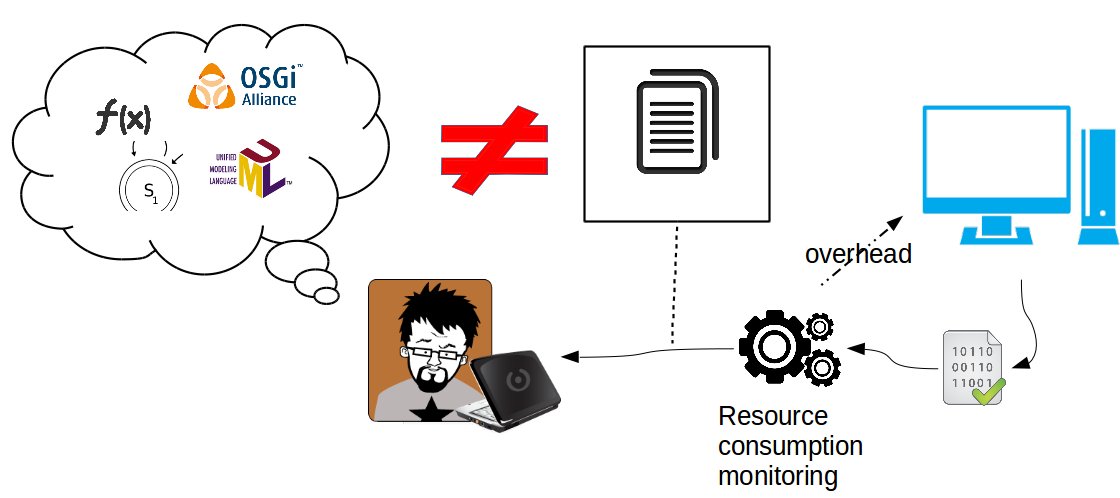
\includegraphics[scale=0.3]{fig/problems.png}
		\end{figure}
		\begin{center}
			\textcolor{red}{\large We need \underline{efficient} development \underline{tools}}
		\end{center}
	\end{frame}
	
	% DONE - 6
%	\begin{frame}{Objectives}
%		\begin{enumerate}
%			\item Support resource Consumption Monitoring and Reservation in MRTEs
%			\begin{itemize}
%				\item Handle many types of resource
%				\item Portable
%				\item Low overhead
%			\end{itemize}
%			\vspace{0.5cm}
%			\item Provide support using the same concepts that developers \tikz[remember picture] \node (a) {\vphantom{X}};
%			\begin{itemize}
%				\item Dealing with abstraction-specific requirements
%				\item Easing the construction of resource management tools for specific software abstractions
%			\end{itemize}
%		\end{enumerate}
%		\begin{tikzpicture}[remember picture,overlay]
%		\path (a.east) ++(-2,-2) node[anchor=west,cloud callout,fill=red!50,opacity=.5, callout absolute pointer={(a.east)}, text width = 2cm]
%		{
%			{\tiny
%				Applications are composed by parts
%				built using abstractions.\\[0.3cm]
%				Can we detect the consumption of each part?\\
%			}
%		};
%		\end{tikzpicture}
%	\end{frame}
	
	\section[State of the Art]{State of the Art}
	
	% DONE - 7
	\begin{frame}{Resource Consumption Monitoring and Reservation in MRTEs}
		\vspace{-.3cm}
		\begin{block}<2->{}
			\uncover<4->{
\includegraphics[scale=0.2]{fig/ys.png}~Arbitrary structures} \hfill 
\includegraphics[scale=0.2]{fig/bs.png}~All resource types
		\end{block}
		\begin{columns}
			\column{0.48\textwidth}
			\begin{scriptsize}
				\begin{block}{\textbf{OS Specific} \hfill \textcolor{red}{low overhead}}
					\begin{itemize}
						\item Cgroups\uncover<2->{~
\includegraphics[scale=0.2]{fig/bs.png}}
						\item Overseer (HPC)
						\item Resource Containers\uncover<2->{~
\includegraphics[scale=0.2]{fig/bs.png}}
						\item Jails\uncover<2->{~
\includegraphics[scale=0.2]{fig/bs.png}}
						\item Jamus\uncover<2->{~
\includegraphics[scale=0.2]{fig/bs.png}}
					\end{itemize}
					\vfill
				\end{block}
			\end{scriptsize}  
			\column{0.48\textwidth}
			\begin{scriptsize}
				\begin{block}<3->{\textbf{MRTE Specific} \hfill \textcolor{red}{low--medium overhead}}
					\begin{itemize}
						\item MVM
						\item KaffeOS
						\item Modified GC
						\item Dynamic Profiling~
\includegraphics[scale=0.2]{fig/bs.png}\uncover<4->{
\includegraphics[scale=0.2]{fig/ys.png}}
						\item OSGi Memory Profiling
						\item Tracing Objects
					\end{itemize}
				\end{block}
			\end{scriptsize}
		\end{columns}
		\begin{columns}
			\column{0.6\textwidth}
			\begin{scriptsize}
				\begin{block}<5->{\textbf{Application level (portable)} \hfill \textcolor{red}{medium-high overhead}}
					\begin{itemize}
						\item JRes~
\includegraphics[scale=0.2]{fig/bs.png}
						\item JRAF2
						\item Instrumentation-based monitoring~
\includegraphics[scale=0.2]{fig/bs.png}
\includegraphics[scale=0.2]{fig/ys.png}
						\item OSGi CPU Profiling
						\item Multi-tenant CPU isolation
					\end{itemize}
				\end{block}
			\end{scriptsize}
		\end{columns}
		%\centering{
		%	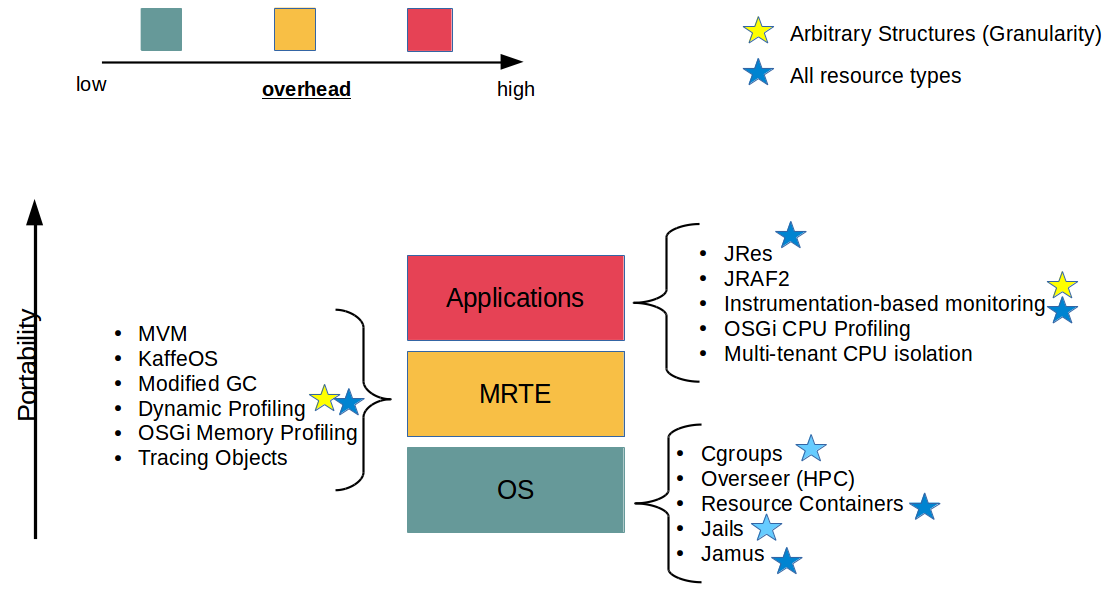
\includegraphics[scale=0.33]{fig/state-of-the-art.png}
		%}
		\uncover<5->{
			\centering{
				\color{red} Instrumentation-based monitoring is \underline{almost} good\\
				{
					\scriptsize Can also be used as the foundation for reservation \\
			%		{\color{black} \dots and the {\color{yellow} \underline{\textbf{star}}} is important}
				} 
			}
		}
	\end{frame}
	
	% DONE - 8
%	\begin{frame}{Approaches to deal with abstraction specific features}
%		\textbf{Facts:}
%		\begin{footnotesize}
%			\begin{itemize}
%				\item Software is built using abstractions
%				\item \textit{Threads}, \textit{Processes}, \textit{classes}, \textit{objects}
%				\item \dots but also: \textit{components} and other \textit{domain-specific abstractions}
%				\item Developers want to see analyze resource usage using their \textit{abstractions}
%			\end{itemize}
%		\end{footnotesize}
%		\vspace{0.5cm}
%		{\centering
%			\color{red} How to \underline{efficiently} support resource-awareness in the presence of abstractions?\\
%		}
%		\vspace{0.5cm}
%		\textbf{Problems}
%		\begin{footnotesize}
%			\begin{enumerate}[i]
%				\item Have unique features
%				\item Tools to support resource awareness are hard to reuse
%				\item lack of tools when new abstractions are defined
%				\item re-implement tools vs extensible tools
%			\end{enumerate}
%		\end{footnotesize}
%		%\textbf{Related works:}
%		%\begin{footnotesize}
%		%	\begin{itemize}
%		%		\item Profiling
%		%		\item Static Analysis
%		%		\item Tooling support for DSLs
%		%	\end{itemize}
%		%\end{footnotesize}
%	\end{frame}
	
	% DONE - 9
	\begin{frame}{Easing the construction of resource management tools}
		\framesubtitle{Relevance of approaches}
		\centering{
			\newcommand{\asymcloud}[2][.1]{%
\begin{scope}[#2]
\pgftransformscale{#1}%    
\pgfpathmoveto{\pgfpoint{261 pt}{115 pt}} 
  \pgfpathcurveto{\pgfqpoint{70 pt}{107 pt}}
                 {\pgfqpoint{137 pt}{291 pt}}
                 {\pgfqpoint{260 pt}{273 pt}} 
  \pgfpathcurveto{\pgfqpoint{78 pt}{382 pt}}
                 {\pgfqpoint{381 pt}{445 pt}}
                 {\pgfqpoint{412 pt}{410 pt}}
  \pgfpathcurveto{\pgfqpoint{577 pt}{587 pt}}
                 {\pgfqpoint{698 pt}{488 pt}}
                 {\pgfqpoint{685 pt}{366 pt}}
  \pgfpathcurveto{\pgfqpoint{840 pt}{192 pt}}
                 {\pgfqpoint{610 pt}{157 pt}}
                 {\pgfqpoint{610 pt}{157 pt}}
  \pgfpathcurveto{\pgfqpoint{531 pt}{39 pt}}
                 {\pgfqpoint{298 pt}{51 pt}}
                 {\pgfqpoint{261 pt}{115 pt}}
\pgfusepath{fill,stroke}         
\end{scope}}  

\begin{figure}[!ht]
\centering
\resizebox{1.01\textwidth}{!}{%
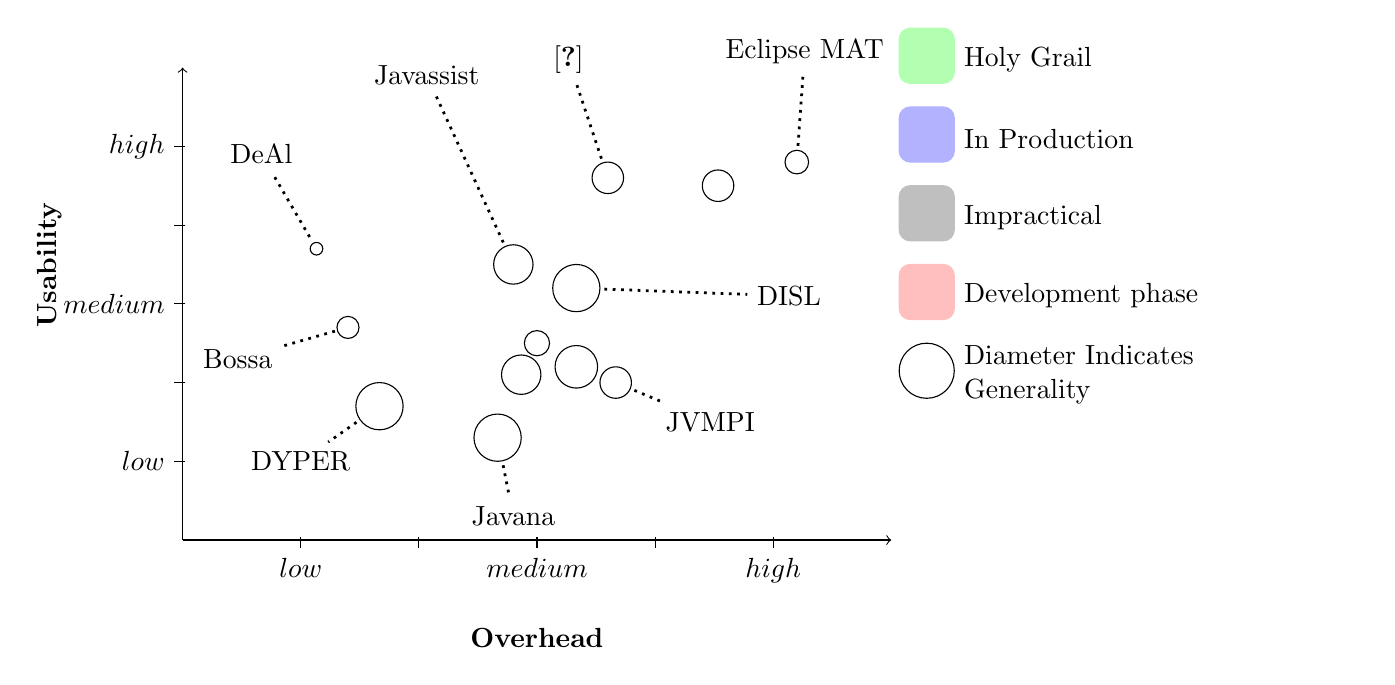
\begin{tikzpicture}
  \draw[->,xshift=0cm] (0,0) -- coordinate (x axis mid) (9,0);
  \draw[->,xshift=0cm] (0,0) -- coordinate (y axis mid) (0,6);
  \foreach \x/\xtext in {1.5/low,3/,4.5/medium,6/,7.5/high}
          \draw [xshift=0cm](\x cm,1pt) -- (\x cm,-3pt)
              node[anchor=north] {$\xtext$};
  \foreach \y/\ytext in {1/low,2/,3/medium,4/,5/high}
          \draw (1pt,\y cm) -- (-3pt,\y cm) node[anchor=east] {$\ytext$}; 
          
  \node[below=1cm] at (x axis mid) {\textbf{Overhead}};
  \node[rotate=90, above left=2cm] at (y axis mid) {\textbf{Usability}};  
  % good region
  \node (cloudgood) at (2,4.9) {\tikz \asymcloud[0.17]{fill=green!30, draw=green!30,thick};};

  %\filldraw[fill=green, draw=green, rounded corners] (0.5,5.5) rectangle (3.5,3);
  
  %bad region
  \node (cloudbad) at (6.3,1.7) {\tikz \asymcloud[0.16]{fill=gray!50, draw=gray!50,thick};};
  
  %useful during development region
  \node (clouddevelopment) at (6.5,4.8) {\tikz \asymcloud[0.17]{fill=pink, draw=pink,thick};};

  %useful in production but not easy to use's region
  \node (cloudproduction) at (2,1.6) {\tikz \asymcloud[0.17]{fill=blue!30, draw=blue!30,thick};};

  % legend
  \filldraw[fill=green!30, draw=green!30, rounded corners] (9.1,6.5) rectangle (9.8,5.8);
  \node[right=0.7cm] at (9.1,6.1) {Holy Grail};
  
  \filldraw[fill=blue!30, draw=blue!30, rounded corners] (9.1,5.5) rectangle (9.8,4.8); 
  \node[right=0.7cm] at (9.1,5.1) {In Production};
  
  \filldraw[fill=gray!50, draw=gray!50, rounded corners] (9.1,4.5) rectangle (9.8,3.8);
  \node[right=0.7cm] at (9.1,4.1) {Impractical};
  
  \filldraw[fill=pink, draw=pink, rounded corners] (9.1,3.5) rectangle (9.8,2.8);
  \node[right=0.7cm] at (9.1,3.1) {Development phase};
  
  \draw (9.45,2.15) circle [radius=0.35];
  \node[right=0.7cm, text width = 5cm, align=left] at (9.1,2.1) {Diameter Indicates\\ Generality};
  
  % very general radius = 0.3
  % general radius = 0.2
  % limited radius = 0.1
  
  % JVMPI - medium usability - high overhead - average generality
  \draw[draw=black] (5.5,2) circle [radius=0.2cm];
  \path (5.5,2) node[circle,minimum size=0.5cm](JVMPI) {}
  		(6.7,1.5) node(JVMPIT) {JVMPI};
  \draw[draw=black,dotted, line width = 1pt] (JVMPI) -- (JVMPIT);
  %\node at (0.5,5.5) {\cite{Liang1999}};
  
  % JAVANA - low usability - medium overhead - high generalidad
  \draw[draw=black] (4,1.3) circle [radius=0.3cm];
  \path (4,1.3) node[circle,minimum size=0.7cm](JAVANA) {}
    		(4.2,0.3) node(JAVANAT) {Javana};
  \draw[draw=black,dotted, line width = 1pt] (JAVANA) -- (JAVANAT);
  
  % Binder CPU Profiling - medium overhead - medium/low usabilityc - low/medium generalidad 
  \draw[draw=black] (4.5,2.5) circle [radius=0.16cm]; % no
  
  % DYPER - medium/low overhead - low usability - high generalidad
  \draw[draw=black] (2.5, 1.7) circle [radius=0.3cm];
  \path (2.5, 1.7) node[circle,minimum size=0.7cm](DYPER) {}
      		(1.5,1) node(DYPERT) {DYPER};
  \draw[draw=black,dotted, line width = 1pt] (DYPER) -- (DYPERT);
  
  % ASM - medium overhead - low/medium usability - high generalidad
  \draw[draw=black] (4.3,2.1) circle [radius=0.25cm]; % [above=0.1]-- (2.3,2.7) node {ASM};
  
  % Javaassist - medium overhead - medium/high usability - high generality
  \draw[draw=black] (4.2,3.5) circle [radius=0.25cm];
  \path (4.2,3.5) node[circle,minimum size=0.6cm](Javassist) {}
        		(3.1,5.9) node(JavassistT) {Javassist};
  \draw[draw=black,dotted, line width = 1pt] (Javassist) -- (JavassistT);
  
  % Profiling with AspectJ - high usability - high overhead - averagage generality
  \draw[draw=black] (6.8,4.5) circle [radius=0.2cm]; % [above=0.1]-- (6.3,5) node {\cite{Pearce:2007:PA:1248445.1248448}};
  
  % Binder Major/AspectJ - medium overhead - high usability - average generalidad
  \draw[draw=black] (5.4,4.6) circle [radius=0.2cm];
  \path (5.4,4.6) node[circle,minimum size=0.5cm](Major) {}
          		(4.9,6.1) node(MajorT) {\cite{Binder:2006:FEM:1173706.1173733}};
  \draw[draw=black,dotted, line width = 1pt] (Major) -- (MajorT);
  
  % DISL - medium overhead - medium usability - full generalidad
  \draw[draw=black] (5,3.2) circle [radius=0.3cm];
  \path (5,3.2) node[circle,minimum size=0.7cm](DISL) {}
        (7.7,3.1) node(DISLT) {DISL};
  \draw[draw=black,dotted, line width = 1pt] (DISL) -- (DISLT);
  
  % Customized aspect weavers - medium overhead - low usability - full generalidad
  \draw[draw=black] (5, 2.2) circle [radius=0.27cm];
  
  % Eclipse MAT/ Visual VM/ YourKit - high overhead - meidum/high usability - limited/medium
  \draw[draw=black] (7.8,4.8) circle [radius=0.15cm];
  \path (7.8,4.8) node[circle,minimum size=0.4cm](Eclipse) {}
        (7.9,6.2) node(EclipseT) {Eclipse MAT};
  \draw[draw=black, dotted, line width = 1pt] (Eclipse) -- (EclipseT);
  
  % DeAl - low overhead - medium/high usability - limited generalidad
  \draw[draw=black] (1.7,3.7) circle [radius=0.08cm];
  \path (1.7,3.7) node[circle,minimum size=0.17cm](DeAl) {}
        (1,4.9) node(DeAlT) {DeAl};
  \draw[draw=black, dotted, line width = 1pt] (DeAl) -- (DeAlT);
  
  % DeAl - low/medium overhead - medium usability - limited generalidad
  \draw[draw=black] (2.1,2.7) circle [radius=0.14cm];
  \path (2.1,2.7) node[circle,minimum size=0.17cm](Bossa) {}
      (0.7,2.3) node(BossaT) {Bossa};
  \draw[draw=black, dotted, line width = 1pt] (Bossa) -- (BossaT);
  
\end{tikzpicture}
}
\caption{\scriptsize Area of circumference indicates how general the approach is (the larger the better)}
\end{figure}

		}
	\end{frame}
	
	
	\begin{frame}{Synthesis}
		\begin{block}{On resource consumption monitoring and reservation for MRTEs}
			\begin{footnotesize}
				\begin{itemize}
					\item There are many approaches with different overhead and accuracy
					\item Most approaches are not portable, but they offer low-medium overhead
					\item Portable approaches are not usable in production due to their high overhead
				\end{itemize}
				
			\end{footnotesize}
		\end{block}
		\vspace{1cm}
		\begin{block}{Easing the construction of resource management tools}
			\begin{footnotesize}
				\begin{itemize}
					\item Most easy to use tools are useful during development, but they fail in production environments
					\item Most approaches are nor usable enough nor they offer low performance overhead
				\end{itemize}
				
			\end{footnotesize}
		\end{block}
	\end{frame}
	
	\section[Contributions]{Contributions}
	
	% DONE ? - 10
	\begin{frame}{Contributions}
		%\framesubtitle{ Synthesis and relation to contributions }
			
			\begin{block}{{\large 1 -- Scapegoat}}
				An adaptive resource consumption monitoring framework for component-based systems.
			\end{block}
%			
%			\begin{columns}
%				\column{.57\textwidth}
%				\begin{itemize}
%					\item Lack of portable, efficient, and generic resource consumption monitoring tools
%				\end{itemize}
%				\column{.01\textwidth}
%				
%				\column{.37\textwidth}
%				\begin{itemize}
%					\item Scapegoat -- an adaptive monitoring framework
%				\end{itemize}
%			\end{columns}
		
		\vspace{0.2cm}
			\begin{scriptsize}
				\begin{block}{\textcolor{gray}{2 -- Squirrel methodology}}
					\textcolor{gray}{An architecture-driven approach to reduce the overhead of resource reservation by choosing the proper mapping to represent components in the runtime.}
				\end{block}
				\begin{block}{\textcolor{gray}{3 -- A domain-specific language to define memory profilers}}
					\textcolor{gray}{A generative approach to ease the construction of tools for supporting resource-aware programming. In particular, it support the construction of profilers that can be used at runtime.}
				\end{block}
			\end{scriptsize}
			
%			\begin{columns}
%				\column{.47\textwidth}
%				\begin{itemize}
%					\item Lack of efficient resource reservation tools for component platforms
%				\end{itemize}
%				\column{.01\textwidth}
%					
%				\column{.47\textwidth}
%				\begin{itemize}
%					\item Squirrel -- an approach to reduce the overhead of resource reservation
%				\end{itemize}
%			\end{columns}
		
 	\end{frame}
	
	% bullet con las conclusiones of state of the art
	
	% slide linking conclusions and contributions
	
	%\begin{frame}{Subway map (Roadmap)}
	%	\newcommand{\placelast}{west}
\newcommand{\placelastt}{south}
\newcommand{\placelasttt}{north}


{
\fontfamily{phv}\selectfont

\begin{figure}[!ht]
\centering

\resizebox{0.9\textwidth}{!}{%
\begin{tikzpicture}

% main railway
\draw[draw=red!70, line width=9pt, cap=round, join=round] (0,0)--(3,-3)--(7.5,-3)--(8.5,-4)--(9.5,-5)--(11,-5);
% abstractions' railway
\draw[draw=blue!40, line width=9pt, cap=round, join=round] (7.5,-4.5)--(5.5,-4.5)--(5.5,-2.65)--(7.5,-2.65)--(9,-1.65)--(10.7,-1.65);
% monitoring railway
\draw[draw=green!40, line width=9pt, cap=round, join=round] (3.95,0.45) -- (2.45,0.45)--(1.25,-0.75)--(2.25,-1.75) -- (3.25,-0.75)--(4.75,-0.75);
% components railway
\draw[draw=pink, line width=9pt, cap=round, join=round] (2,-4.35)--(1,-5.35)--(3,-3.35)--(4.2,-3.35)--(4.2,-4.35)--(4.2,-5.65);

% main railway
\foreach [count=\c] \x/\cy/\text/\place in {
   0/0/{}/east,
   8.5/-4/\parbox{2.5cm}{Ease construction of tools}/west,
   11/-5/\parbox{1.7cm}{Resource awareness}/\placelast
  } {
  
  \filldraw[fill=white, draw=black, line width=1pt] (\x,\cy) circle [radius=0.15];
  \draw[draw=black,dotted, line width = 1pt] (\x,\cy) node[anchor=\place, font=\scriptsize, inner sep=0.3cm] {\text};
}

% abstractions' railway
\foreach [count=\c] \x/\cy/\text/\place in {
   7.5/-4.5/\parbox{1cm}{{Internal DSL}}/north west,
   6.5/-4.5/\parbox{1cm}{{External DSL}}/north,
   5.5/-4.5/\parbox{0.7cm}{{API}}/north,
   7.5/-2.65/\parbox{0.5cm}{{Fluent API}}/south east,
   9/-1.65/\parbox{1.7cm}{Metamodeling}/south,
   10.7/-1.65/\parbox{1.9cm}{{Components}}/\placelast
  } {
  
  \filldraw[fill=white, draw=black, line width=1pt] (\x,\cy) circle [radius=0.15];
  \draw[draw=black,dotted, line width = 1pt] (\x,\cy) node[anchor=\place, font=\scriptsize, inner sep=0.3cm] {\text};
}

% monitoring railway
\foreach [count=\c] \x/\cy/\text/\place in {
   3.95/0.45/{MRTE Modification}/west,
   2.45/0.45/{Instrumentation}/south,
   3.25/-0.75/\parbox{1.6cm}{Adaptive Monitoring}/north west,
   4.75/-0.75/{Sampling}/\placelast
  } {
  
  \filldraw[fill=white, draw=black, line width=1pt] (\x,\cy) circle [radius=0.15];
  \draw[draw=black,dotted, line width = 1pt] (\x,\cy) node[anchor=\place, font=\scriptsize, inner sep=0.3cm] {\text};
}

% component railway
\foreach [count=\c] \x/\cy/\text/\place in {
   2/-4.35/{Contracts}/east,
   1/-5.35/{Kevoree}/east,
   4.2/-4.35/{cgroups}/north east,
   4.2/-5.65/\parbox{2cm}{System\\ Reconfiguration}/\placelasttt
  } {
  
  \filldraw[fill=white, draw=black, line width=1pt] (\x,\cy) circle [radius=0.15];
  \draw[draw=black,dotted, line width = 1pt] (\x,\cy) node[anchor=\place, font=\scriptsize, inner sep=0.3cm] {\text};
}

%joins
\foreach [count=\c] \x/\cy/\text/\place in {
   1.12/-0.88/\parbox{1.6cm}{Resource Accounting}/east,
   2.12/-1.88/\parbox{1.8cm}{Lightweight accounting}/east,
   3/-3.15/\parbox{2cm}{Accounting\\ for components}/east,
   4.2/-3.15/\parbox{2cm}{Reservation for components}/north,
   5.5/-2.85/\parbox{2cm}{Working with\\ Abstractions}/\placelastt
  } {
 
  \filldraw[fill=white, draw=black, line width=0.04cm] (\x,\cy) circle [radius=0.3];
  \filldraw[fill=white, draw=black, line width=0.04cm] (\x,\cy) circle [radius=0.13];

  \draw[draw=black,dotted, line width = 1pt] (\x,\cy) node[anchor=\place, font=\scriptsize, inner sep=0.3cm] {\text};
}

% contributions
\path (8.5,-4) node[anchor=south east, inner sep=-0.04cm] {

\includegraphics[width=20pt, height=20pt]{../library}
}
(3,-3.15) node[anchor=south east, inner sep=-0.01cm] {

\includegraphics[width=20pt, height=20pt]{../library}
}
(4.2,-3.15) node[anchor=south east, inner sep=-0.01cm] {

\includegraphics[width=20pt, height=20pt]{../library}
}
(11,-5) node[anchor=south east, inner sep=-0.06cm] {

\includegraphics[width=20pt, height=20pt]{../goal}
}
;
% indicator of current location
\draw[color=gray,draw=yellow, line width=7 pt] (0,0) circle (0.4cm);
\path
    [
		postaction={
	        decorate,
            decoration={
                raise=-9pt,
                text along path,
                text align/fit to path stretching spaces=true,
                reverse path=true,
                text align/align=center,
                text align/left indent={1cm}, % \pi * radius
                text align/right indent={0.0cm},
                text={|\scriptsize|YOU ARE HERE}
            }
        }
    ]
(0,0) circle (0.6cm);

% legend
\path (11, 1.7) node {
	
\includegraphics[width=20pt, height=20pt]{../goal}
} (12.2,1.6) node {{\scriptsize Objective}}
;
\path (11, 0.9) node {
	
\includegraphics[width=20pt, height=20pt]{../library}
} (12.4,0.8) node {{\scriptsize Contributions}}
;
\draw[line width=0.1cm, draw=red!70] (10.7, 0.2)--(11.3,0.2) (12.4,0.2) node {{\scriptsize Thesis's way}}
;

\draw[line width=0.1cm, draw=pink] (10.7, -0.2)--(11.3,-0.2) (12.7,-0.2) node {{\scriptsize Components' way}};

\draw[line width=0.1cm, draw=green!40] (10.7, -0.6)--(11.3,-0.6) (12.6,-0.6) node {{\scriptsize Accounting way}};

\draw[line width=0.1cm, draw=blue!40] (10.7, -1)--(11.3,-1) (12.7,-1) node {{\scriptsize Abstractions' way}};

\filldraw[fill=white, draw=black, line width=0.04cm] (11,2.4) circle [radius=0.2];
\filldraw[fill=white, draw=black, line width=0.04cm] (11,2.4) circle [radius=0.08];
\draw (12.6,2.4) node[font=\scriptsize] {Topics Converge};

\end{tikzpicture}
}
\caption{This subway map shows how this research contributes to the state-of-the-art on supporting resource-awareness.} \label{fig:subway-map}
\end{figure}

}
	%\end{frame}
	
	\section[Scapegoat -- A monitoring framework for component systems]{Scapegoat -- A monitoring framework}
	
	\subsection[Approach]{Approach}
	% DONE - 11
	\begin{frame}{Overview}
			\textbf{What is the desired behavior?}
			\begin{enumerate}[i]
				\item Precise and lightweight
				\item Detect \underline{faulty} components \tikz[remember picture] \node (b) {\vphantom{y}};
			\end{enumerate}
			
			\vspace{2cm}
			\uncover<2>{
			\textbf{How to achieve that goal?}\tikz[remember picture] \node (a) {\vphantom{X}};
			\begin{itemize}
				\item Global Monitoring by default
				\item Fine-Grained Monitoring only when required \dots
				\begin{enumerate}[i]
					\item Assume some components are more likely to be faulty
					\item Begin with suspected components
				\end{enumerate}
			\end{itemize}
			}
			\begin{tikzpicture}[remember picture,overlay]
			\path<2> (a.east) ++(2.5,0.7) node[anchor=west,cloud callout,fill=red!50,opacity=.5, callout absolute pointer={(a.east)}, text width = 2cm]
				{
					\centering{\underline{Observation:}} \\
					{\scriptsize
					Consumption matters when \\
					the container is running out \\
					of resources \\
					}
				};
			\end{tikzpicture}
			
			\begin{tikzpicture}[remember picture,overlay]
			\path<1-> (b.east) ++(1,0.3) node[anchor=west,ellipse callout,fill=red!50,opacity=.5, callout absolute pointer={(b.mid)}, text width = 3cm]
			{
				\scriptsize
				Consume more than \textit{expected}\\
			};
			\end{tikzpicture}
			
	\end{frame}
	
	% DONE - 12
	\begin{frame}{Main Loop}
		\centering
		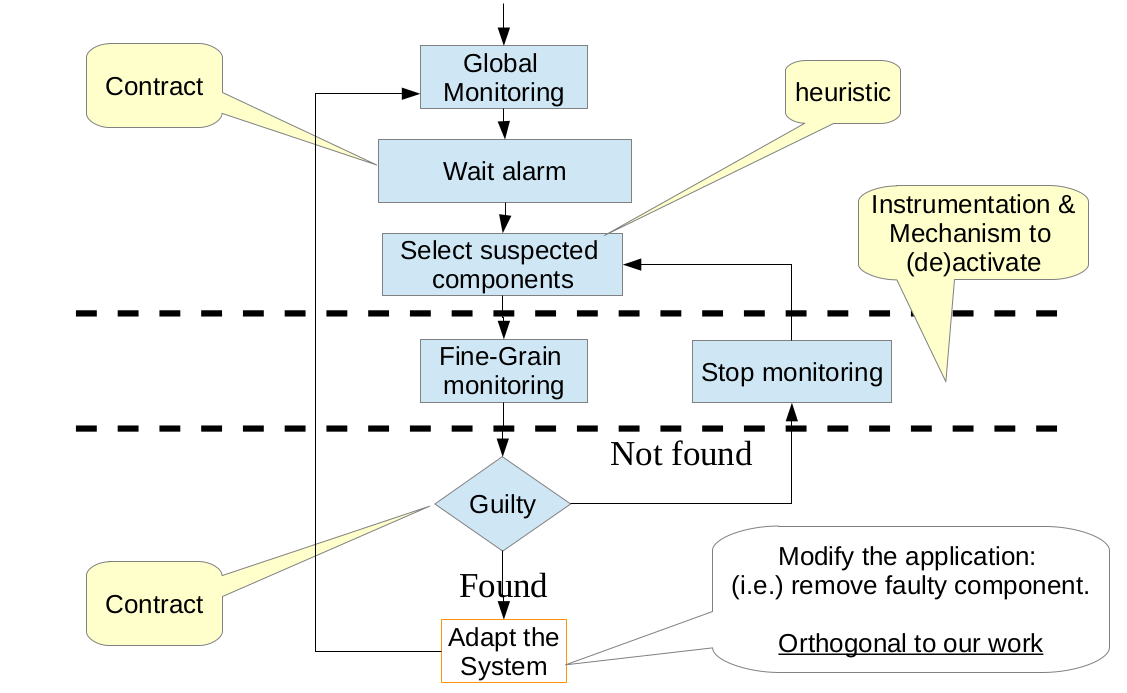
\includegraphics[scale=0.3]{fig/scapegoat.png}
	\end{frame}
	
	% DONE - 13
	\begin{frame}{Contract-based approach}
		\begin{enumerate}
			\item<1-> Contract for the whole system/JVM -- when to trigger the alarm?
					\begin{itemize}
						\item CPU Usage
						\item Memory usage
					\end{itemize}
			\begin{scriptsize}
			\begin{example}[Contract specification for an application]
					\hspace{.5cm} \textbf{add} node0 : JavaNode\\
					\hspace{.5cm} \textbf{set} node0.cpu\_threshold = \textbf{80} \% \\
			\end{example}
			\end{scriptsize}
			\item<2> Contract for each component -- consumption allowed under certain operation conditions
				\begin{itemize}
					\item Peak number of instruction per second
					\item Maximum memory usage
					\item Operation condition %(e.g. If the component receives at most 100 requests per second it consumes at most 30 MB)
				\end{itemize}
				\begin{scriptsize}\begin{example}[Contract specification for a component]
						\hspace{.5cm} \textbf{add} node0.server : WsServer\\
						\hspace{.5cm} \textbf{set} server.cpu\_wall\_time = \textbf{2580323} intr/sec \\
						\hspace{.5cm} \textbf{set} server.memory\_max\_size = \textbf{15000} bytes\\
						\hspace{.5cm} \textbf{set} server.throughput\_all\_ports = \textbf{10000} msg/sec {\color{Emerald} \# operation condition} \\
				\end{example}
				\end{scriptsize}
		\end{enumerate}
		
	\end{frame}
	
	% DONE - 14
	\begin{frame}{Extending the framework with heuristics}
		\uncover{
		\centering{
			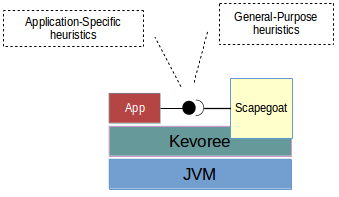
\includegraphics[scale=0.5]{fig/scapegoat-heuristic.png}
		}
		}
		\begin{example}
			\textbf{Number of previous failures}: \\ Components are suspected if they have previously failed
		\end{example}
		\begin{example}
			\textbf{Models@runtime-based heuristic}: Failures come from recent changes
			\begin{itemize}
				\item Recently added components
				\item Components that interact with recently added components
			\end{itemize}
		\end{example}
	\end{frame}
	
	% DONE - 15
	\begin{frame}{Mechanisms to perform monitoring}
		%{
		\begin{footnotesize}
			\begin{alertblock}{Global Monitoring}
				To perform global monitoring we use JMX
			\end{alertblock}
		\end{footnotesize}
		\begin{footnotesize}
			\begin{alertblock}{Memory Consumption Monitoring}
				\begin{itemize}
					\item Instrumentation-based monitoring
					\item Using the JVMTI to explore the Java heap
				\end{itemize}
			\end{alertblock}
		\end{footnotesize} 
		\begin{alertblock}{Switching from global monitoring to fine-grain monitoring}
			\begin{figure}
				\centering
				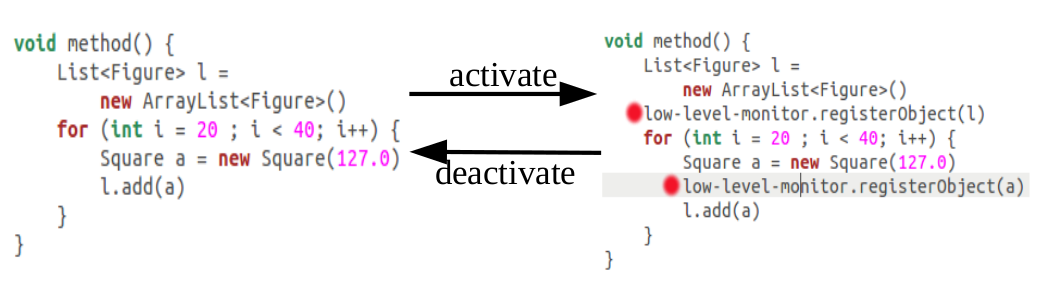
\includegraphics[scale=0.27]{fig/activate-deactivate.png}
			\end{figure}
			\vspace{-.5cm}
			\begin{footnotesize}
				Require Java Agent for:
				\begin{enumerate}[i]
					\item Instrumenting bytecode
					\item Retransforming every class within a component
				\end{enumerate}
			\end{footnotesize}
		\end{alertblock}
	\end{frame}
	
	\subsection[Evaluation]{Evaluation}
	% DONE - 16
	\begin{frame}{Research Questions}
		\begin{enumerate}[RQ1]\setlength{\itemsep}{0.5cm}
			\item What is the impact of the various level of instrumentation?
			\item What are the costs of using instrumentation-based memory monitoring and heap exploration?  
			\item Does adaptive  monitoring outperform state-of-the-art instrumentation monitoring?
			\item What is the impact of application size (i.e. number of components, size of components) and the quality of the heuristic?
			\begin{enumerate}[a]
				\item Execution time
				\item Time to discover faulty components
			\end{enumerate}
		\end{enumerate}
		\vfill
	\end{frame}
	
	% DONE - 17
	\begin{frame}{Overhead of the instrumentation solutions}
		{} \tikz[remember picture] \node (a) {\vphantom{y}};
		
		\begin{tikzpicture}[remember picture,overlay]
		\path (a.east) ++(8.7,-.5) node[anchor=west,ellipse,fill=red!50,opacity=.5, text width = 2.5cm]
		{
			{\scriptsize
				\centering{\underline{RQ1}}: \\
				What is the impact of the various level of instrumentation? \\
			}
		};
		\end{tikzpicture}
		
		\begin{figure}[!ht]
\centering
\resizebox{0.8\textwidth}{!}{%
\begin{tikzpicture}
\begin{axis}[
every axis legend/.append style={nodes={right}},
ybar=0pt,
legend style={at={(0.25,1.1)},
anchor=north,legend columns=1, font=\tiny},
ylabel={Time (seconds)},
y label style={at={(0.04, 0.5)}},
scaled y ticks = false,
      y tick label style={/pgf/number format/fixed, font=\scriptsize,
      /pgf/number format/1000 sep = \thinspace % Optional if you want to replace comma as the 1000 separator 
      },
xtick=data,ymin=0,
width = 13cm,
height = 5cm,
bar width = 6,
x tick label style={rotate=45,anchor=east, font=\scriptsize},
 axis lines*=left, % Don't display the top and right lines
 symbolic x coords={antlr,fop,hsqldb,jython,chart,luindex,xalan,lusearch}
]
\addplot[fill=black] coordinates 
	{(antlr,1.28) (fop,1.101) (hsqldb,2.337) (jython,2.351) (chart,2.534) (luindex,3.561) (xalan,1.224) (lusearch,1.305)};
\addplot[fill=gray] coordinates 
	{(antlr,1.023) (fop,1.039) (hsqldb,2.284) (jython,2.524) (chart,2.417) (luindex,3.165) (xalan,1.191) (lusearch,1.321)};
\addplot[pattern=north east lines] coordinates 
	{(antlr,2.164) (fop,1.188) (hsqldb,8.655) (jython,10.688) (chart,4.806) (luindex,8.001) (xalan,4.885) (lusearch,9.349)};
\addplot[pattern=crosshatch] coordinates 
	{(antlr,6.235) (fop,1.905) (hsqldb,9.091) (jython,10.905) (chart,8.985) (luindex,44.988) (xalan,8.026) (lusearch,9.261)};
\addplot[pattern=dots] coordinates 
	{(antlr,7.468) (fop,1.970) (hsqldb,15.888) (jython,18.625) (chart,11.502) (luindex,51.660) (xalan,11.188) (lusearch,18.975)};
\legend{\underline{\textit{No monitoring}}, Global monitoring, \underline{Memory instrumentation},\underline{Instructions instrumentation}, Memory \& Instructions instrumentation}
\end{axis}
\end{tikzpicture}
}
\caption{\scriptsize Execution time for tests using the DaCapo Benchmark\label{overhead-of-monitoring}}
\end{figure}
		
		\centering{
			\normalsize
			\color{red} {
				 Memory instrumentation, average overhead of 329\% \\
				 Instruction instrumentation, average overhead  of 562\% \\
			}
		}
	\end{frame}
	
	% DONE - 18
	\begin{frame}{Instrumentation-based memory monitoring vs. heap exploration-based memory monitoring}
		{} \tikz[remember picture] \node (a) {\vphantom{y}};
		\begin{tikzpicture}[remember picture,overlay]
		\path (a.east) ++(8.7,-.5) node[anchor=west,ellipse,fill=red!50,opacity=.5, text width = 2.5cm]
		{
			{\scriptsize
				\centering{\underline{RQ2}}: \\
				What are the costs of using instrumentation-based memory monitoring and heap exploration? \\
			}
		};
		\end{tikzpicture}
		\begin{figure}[!ht]
\centering
\resizebox{0.8\textwidth}{!}{%
\begin{tikzpicture}
\begin{axis}[
every axis legend/.append style={nodes={right}},
ybar=0pt, legend style={at={(0.28,1.1)},
anchor=north,legend columns=1, font=\tiny},
ylabel={Time (seconds)},
y label style={at={(0.04, 0.5)}},
scaled y ticks = false,
      y tick label style={/pgf/number format/fixed, font=\scriptsize,
      /pgf/number format/1000 sep = \thinspace % Optional if you want to replace comma as the 1000 separator 
      },
xtick=data,ymin=0,
width = \textwidth,
height = 5cm,
bar width = 6,
x tick label style={rotate=45,anchor=east, font=\scriptsize},
 axis lines*=left, % Don't display the top and right lines
 symbolic x coords={antlr,fop,hsqldb,jython,chart,luindex,xalan,lusearch}
]
% no monitoring
\addplot[fill=black] coordinates 
	{(antlr,1.28) (fop,1.101) (hsqldb,2.337) (jython,2.351) (chart,2.534) (luindex,3.561) (xalan,1.224) (lusearch,1.305)};
% memory
\addplot[pattern=north east lines] coordinates 
	{(antlr,2.164) (fop,1.188) (hsqldb,8.655) (jython,10.688) (chart,4.806) (luindex,8.001) (xalan,4.885) (lusearch,9.349)};
% heap dump
\addplot[fill=gray] coordinates 
	{(antlr,1.143) (fop,1.125) (hsqldb,8.639) (jython,2.762) (chart,2.836) (luindex,3.589) (xalan,1.822) (lusearch,5.078)};
% memory and instructions
\addplot[pattern=dots] coordinates 
	{(antlr,7.468) (fop,1.970) (hsqldb,15.888) (jython,18.625) (chart,11.502) (luindex,51.660) (xalan,11.188) (lusearch,18.975)};
% heap dump and instructions
\addplot[fill=white] coordinates 
	{(antlr,6.159) (fop,1.188) (hsqldb,14.647) (jython,10.950) (chart,9.059) (luindex,44.758) (xalan,7.812) (lusearch,15.990)};
% legend
\legend{\underline{\textit{No Monitoring}}, \underline{Memory instrumentation}, \underline{Heap Exploration}, Memory \& Instructions instrumentation, Heap Exploration \& Instructions Instrumentation}
\end{axis}
\end{tikzpicture}
}
\caption{\scriptsize Using different memory monitoring techniques}
\end{figure}

		\centering{
			\color{red} {Memory Instrumentation $=>$ average overhead of 329\% \\ Heap Exploration $=>$ average overhead of 179\%}
		}
	\end{frame}
	
	% DONE - 19
	\begin{frame}{Overhead of Adaptive Monitoring vs Components Instrumented all the time}
		\framesubtitle{Experiment Setting}
		\begin{itemize}
			\item Components of firefighter use case (13 components)
			\item One component that \underline{fails over and over} \tikz[remember picture] \node (a) {\vphantom{X}};
			\item Component with a job to complete -- used to measure its execution time
		\end{itemize}
		\begin{tikzpicture}[remember picture,overlay]
		\path (a.east) ++(1.5,.7) node[anchor=west,ellipse callout,fill=red!50,opacity=.5, callout absolute pointer={(a.east)}, text width = 2.5cm]
		{
			
			{\scriptsize
				\centering{\underline{Worst-case scenario:}} \\
				Switching states \\
				Global \\
				Fine-Grain \\
				Global \\
				Fine-Grain \\
				\dots \\
			}
		};
		\end{tikzpicture}
		
		\begin{tiny}
			\begin{table}[!hb]
				\centering
				\caption{Setting of use cases}
				\begin{tabular}{p{0.5cm}|p{1.35cm}p{0.85cm}p{2.5cm}p{2.5cm}}
					\hline \textbf{Test Name} & \textbf{Monitored\newline Resource} & \textbf{Faulty\newline Resource} & \textbf{Heuristic} & \textbf{External Task} \\ 
					\hline \hline UC1 & CPU, Memory & CPU & number of failures & Weka, train neural network \\ 
					UC2 & CPU, Memory & CPU & number of failures & dacapo, antlr \\ 
					UC3 & CPU, Memory & CPU & number of failures & dacapo, chart \\ 
					UC4 & CPU & CPU & number of failures & dacapo, xalan \\ 
					UC5 & CPU, Memory & CPU & less number of failures first  & dacapo, chart \\ 
					UC6 & Memory & CPU & number of failures & Weka, train neural network \\ 
					\hline 
				\end{tabular} 
			\end{table}
		\end{tiny}
	\end{frame}
	
	% DONE - 20
	\begin{frame}{Overhead of Adaptive Monitoring vs Components Instrumented all the time}
		\framesubtitle{Experiment Results}
		{} \tikz[remember picture] \node (a) {\vphantom{y}};
		\begin{tikzpicture}[remember picture,overlay]
		\path (a.east) ++(8.7,-.5) node[anchor=west,ellipse,fill=red!50,opacity=.5, text width = 2.5cm]
		{
			{\scriptsize
				\centering{\underline{RQ3}}: \\
				Does adaptive  monitoring outperform state-of-the-art instrumentation-based monitoring? \\
			}
		};
		\end{tikzpicture}
		\begin{figure}
\centering
\resizebox{0.8\textwidth}{!}{%
\begin{tikzpicture}
\begin{axis}[
every axis legend/.append style={nodes={right}},
ybar=0pt, legend style={at={(0.4,1.2)},
anchor=north,legend columns=1, font=\tiny},
ylabel={Time (seconds)},
y label style={at={(0.02, 0.5)}},
scaled y ticks = false,
      y tick label style={/pgf/number format/fixed,font=\scriptsize,
      /pgf/number format/1000 sep = \thinspace % Optional if you want to replace comma as the 1000 separator 
      },
xtick=data,ymin=0,
width = \textwidth,
height = 5cm,
bar width = 6,
x tick label style={rotate=45,anchor=east, font=\scriptsize},
 axis lines*=left, % Don't display the top and right lines
 symbolic x coords={UC1,UC2,UC3,UC4,UC5,UC6}
]
% full monitoring
\addplot[fill=black] coordinates 
	{(UC1,613.000) (UC2,46.363) (UC3,63.899) (UC4,78.324) (UC5,49.144) (UC6,132.949)};
% adaptive with all component
\addplot[fill=red, pattern=crosshatch dots] coordinates 
	{(UC1,432.744) (UC2,70.501) (UC3,198.554) (UC4,187.036) (UC5,32.340) (UC6,127.711)};
% adaptive with all component and heap dump
\addplot[fill=yellow, pattern=crosshatch] coordinates 
	{(UC1,410.790) (UC2,61.808) (UC3,95.503) (UC4,204.479) (UC5,16.864) (UC6,123.381)};
% adaptive with heuristic
\addplot[fill=green, pattern=north west lines] coordinates 
	{(UC1,176.413) (UC2,16.741) (UC3,29.461) (UC4,19.470) (UC5,27.001) (UC6,123.813)};
% adaptive with heuristic and heap dump
\addplot[fill=pink, pattern=dots] coordinates 
	{(UC1,169.467) (UC2,12.520) (UC3,16.403) (UC4,20.251) (UC5,15.110) (UC6,124.294)};
% global monitoring
\addplot[fill=cyan, pattern=north east lines] coordinates 
	{(UC1,166.759) (UC2,10.646) (UC3,14.37) (UC4,20.860) (UC5,14.77) (UC6,120.16)};
\legend{
	\underline{Components Instrumented all the time}, 
	Adaptive with All Components using Memory Instrumentation, 
	Adaptive with All Components using Heap Exploration, 
	Localized monitoring using Memory Instrumentation, 
	\underline{Localized monitoring using Heap Exploration},
	Global Monitoring}
\end{axis}
\end{tikzpicture}
}
%\caption{Execution time for some use cases under different monitoring policies.}\label{adaptive-vs-full}
\end{figure}

		\centering{
			\color{red}
			Components Instrumented all the time vs Adaptive Monitoring:\\ \underline{Overhead Reduced by 93\% on average}
		}
	\end{frame}
	
	% DONE - 21
	\begin{frame}{Impact of application size and heuristic on \underline{execution time}}
		{} \tikz[remember picture] \node (a) {\vphantom{y}};
		\begin{tikzpicture}[remember picture,overlay]
		\path (a.east) ++(8.7,-.5) node[anchor=west,ellipse,fill=red!50,opacity=.5, text width = 2.5cm]
		{
			{\scriptsize
				\centering{\underline{RQ4a}}: \\
				What is the impact of application size and the quality of the heuristic on execution time? \\
			}
		};
		\end{tikzpicture}
		{}\\
		\textbf{Experiment setup:}
		\begin{scriptsize}
			\begin{itemize}
				\item Faulty component that fails over and over
				\item Component with a job to complete -- to measure its execution time
				\item Variable number of components: 4, 8, 16, 32, 64, 128
				\item Perfect Heuristic: \textit{Number of previous failures}
			\end{itemize}
		\end{scriptsize}
		 \begin{figure}
 \centering
\resizebox{0.7\textwidth}{!}{
 % 115 classes
 \begin{minipage}[t]{0.45\linewidth}
 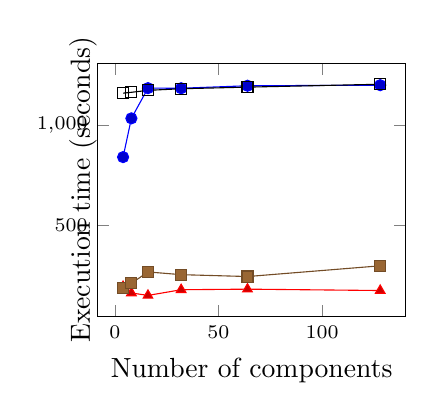
\begin{tikzpicture}
 \begin{axis}[
 	ylabel={Execution time (seconds)},
 	y label style={at={(0.03, 0.5)}},
 	xlabel={Number of components},width = 5.5cm,
 	height = 4.8cm,
 	x tick label style={font=\scriptsize},
 	y tick label style={font=\scriptsize}]

 \addplot+[mark=*] coordinates
 	{(4,842.274) (8,1035.734) (16,1186.657) (32,1186.140) (64,1198.539) (128,1201.415)};
 	
 \addplot+[mark=triangle*] coordinates
 	{(4,195.609) (8,163.964) (16,151.637) (32,180.026) (64,182.962) (128,176.101)};
 	
 \addplot+[mark=square*] coordinates
	 	{(4,186.798) (8,211.913) (16,268.908) (32,255.329)  (64,245.976) (128,299.516)};
	 	
 \addplot+[mark=square] coordinates
	 	{(4,1161.593) (8,1165.910) (16,1175.643) (32,1183.620)  (64,1191.749) (128,1206.128)};
 \end{axis}
 \end{tikzpicture}
 \caption{\scriptsize 115 classes per component}
\end{minipage}
\hspace{0.1\linewidth}
 % 4 classes
 \begin{minipage}[t]{0.45\linewidth}
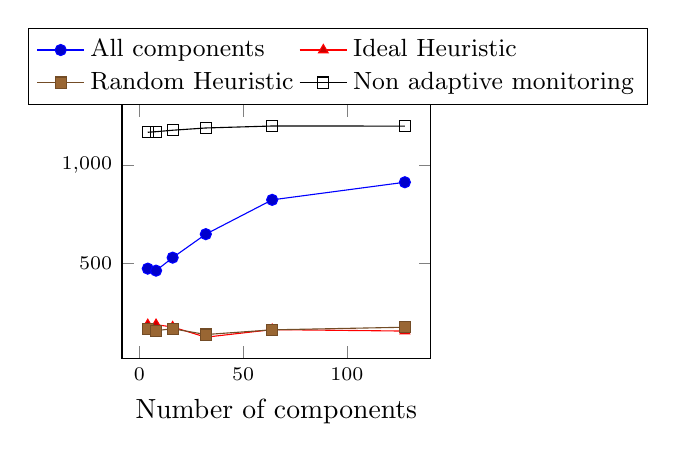
\begin{tikzpicture}
 \begin{axis}[
 	every axis legend/.append style={nodes={right}},
 	legend columns=2,
 	legend style={at={(0.7,1)},
 	anchor=south,legend columns=1, font=\small},
 	xlabel={Number of components},width = 5.5cm,
 	height = 4.8cm,
 	x tick label style={font=\scriptsize},
 	y tick label style={font=\scriptsize}
 	]

\addplot+[mark=*] coordinates
 	{(4,471.532) (8,461.274) (16,527.667) (32,647.634) (64,822.767) (128,912.634)};
 	
 \addplot+[mark=triangle*] coordinates
 	{(4,185.003) (8,185.533) (16,173.457) (32,121.551) (64,160.201) (128,152.802)};
 	
 \addplot+[mark=square*] coordinates
	 	{(4,161.985) (8,154.983) (16,164.704) (32,135.131)  (64,159.032) (128,172.392)};
	 	
 \addplot+[mark=square] coordinates
	 	{(4,1167.814) (8,1170.811) (16,1178.219) (32,1189.748)  (64,1199.834) (128,1199.453)};

	\legend{All components, Ideal Heuristic, Random Heuristic, Non adaptive monitoring}
 \end{axis}
 \end{tikzpicture}
 \caption{\scriptsize Four classes per component}
 \end{minipage}
}
\end{figure}

		\centering{
			\color{red} Heuristic has \underline{limited effect} on execution time 
		}
	\end{frame}
	
	% DONE - 22
	\begin{frame}{Impact of application size and heuristic on \underline{delay time}}
		{} \tikz[remember picture] \node (a) {\vphantom{y}};
		\begin{tikzpicture}[remember picture,overlay]
		\path (a.east) ++(8.7,-.5) node[anchor=west,ellipse,fill=red!50,opacity=.5, text width = 2.5cm]
		{
			{\scriptsize
				\centering{\underline{RQ4b}}: \\
				What is the impact of application size and the quality of the heuristic on time to discover failure? \\
			}
		};
		\end{tikzpicture}
		{}\\
		\textbf{Experiment setup:}
		\begin{scriptsize}
		\begin{itemize}
			\item Same setting as before
			\item \textbf{Delay Time}: Time to discover faulty component.
		\end{itemize}
		\end{scriptsize}
		\begin{figure}
 \centering
\resizebox{0.8\textwidth}{!}{
 % 115 classes
\begin{minipage}[t]{0.45\linewidth}
	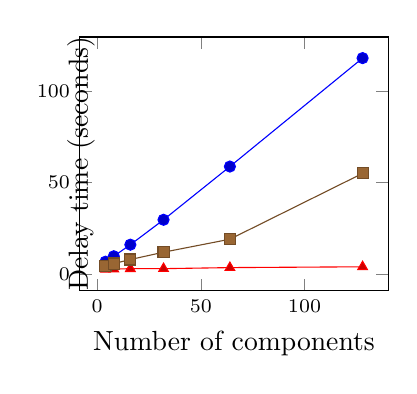
\begin{tikzpicture}
	 \begin{axis}[
	 	ylabel={Delay time (seconds)},
	 	y label style={at={(0.08, 0.5)}},
	 	xlabel={Number of components},width = 5.5cm,
	 	height = 4.8cm,
	 	x tick label style={font=\scriptsize},
	 	y tick label style={font=\scriptsize}]
	
	 \addplot+[mark=*] coordinates
	 	{(4,6.614953125) (8,9.60012962962963) (16,15.9376486486486) (32,29.564) (64,58.7045) (128,118.061571428571)};
	 	
	 \addplot+[mark=triangle*] coordinates
	 	{(4,2.46368292682927) (8,2.56517142857143) (16,2.79086206896552) (32,2.81322222222222) (64,3.3868064516129) (128,3.83251724137931)};
	 	
	 \addplot+[mark=square*] coordinates
		 	{(4,4.31777777777778) (8,5.59077777777778) (16,7.81511538461538) (32,11.8165)  (64,18.9216363636364) (128,54.9538)};
	
	 \end{axis}
	\end{tikzpicture}
\caption{\scriptsize 115 classes per component}
\end{minipage}
\hspace{0.1\linewidth}
 % 4 classes
\begin{minipage}[t]{0.45\linewidth}
	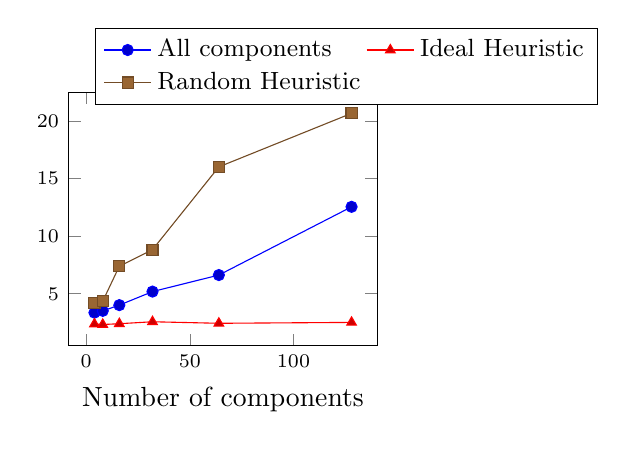
\begin{tikzpicture}
	 \begin{axis}[
	 	every axis legend/.append style={nodes={right}},
	 	legend columns=2, 
	 	legend style={at={(0.9,0.95)},
	 	anchor=south,legend columns=1, font=\small},
	 	xlabel={Number of components},width = 5.5cm,
	 	height = 4.8cm,
	 	x tick label style={font=\scriptsize},
	 	y tick label style={font=\scriptsize}]
	
	 \addplot+[mark=*] coordinates
	 	{(4,3.36101408450704) (8,3.51326153846154) (16,4.01246031746032) (32,5.18675) (64,6.62437704918033) (128,12.5490980392157)};
	 	
	 \addplot+[mark=triangle*] coordinates
	 	{(4,2.3682619047619) (8,2.32882926829268) (16,2.39802777777778) (32,2.568) (64,2.43528571428571) (128,2.51225806451613)};
	 	
	 \addplot+[mark=square*] coordinates
		 	{(4,4.18407692307692) (8,4.35309090909091) (16,7.392) (32,8.82909090909091)  (64,16.017125) (128,20.6681428571429)};
	
		\legend{All components, Ideal Heuristic, Random Heuristic}
	 \end{axis}
	\end{tikzpicture}
%\caption{4 classes}
\caption{\scriptsize Four classes per component}
\end{minipage}
}
\end{figure}

		\centering{
			\color{red} Delay Time \underline{highly affected} by the heuristic 
		}
	\end{frame}
	
	% DONE - 23
%	\begin{frame}{Web use case -- spot faulty components in a scalable diverse web application}
%		\begin{figure}[!bt]
%			\centering
%			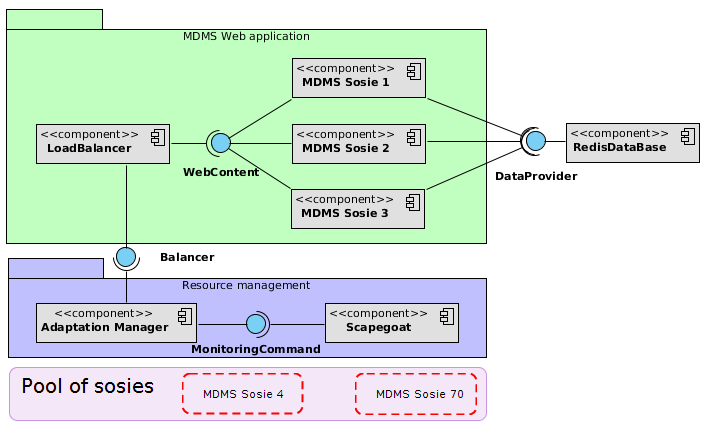
\includegraphics[scale=0.35]{../chapter5/figures/webapp2}
%			\caption{\scriptsize Architecture of MdMS along with Scapegoat and additional components to adapt the system.}
%		\end{figure}
%	\end{frame}
%	
%	% DONE - 24
%	\begin{frame}{Web use case -- spot faulty components in a scalable diverse web application}
%		\begin{figure}
 \centering
\resizebox{0.8\linewidth}{!}{
 \begin{minipage}[t]{0.43\linewidth}
 \centering
 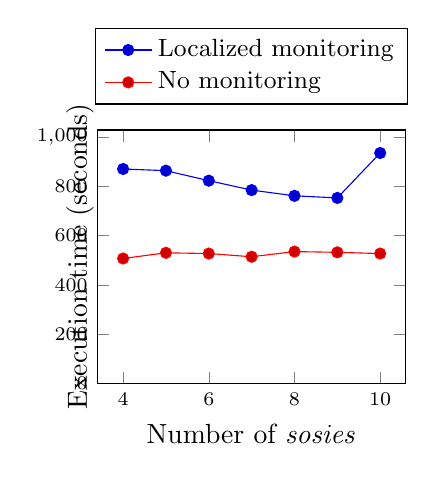
\begin{tikzpicture}
  \begin{axis}[
  	ylabel={Execution time (seconds)},
  	y label style={at={(0.02, 0.5)}},
  	legend style={at={(0.5,1.1)},
  	 	 	anchor=south,legend columns=1, font=\small},
  	ymin=0,
  	every axis legend/.append style={nodes={right}},
  	xlabel={Number of \textit{sosies}},width = 5.5cm,
  	height = 4.8cm,
  	x tick label style={font=\scriptsize},
  	y tick label style={font=\scriptsize}]
 
  \addplot+[mark=*] coordinates
  	{(4, 870.375) (5, 863.5) (6, 822.875) (7, 784.625) (8, 761.375) (9, 752.875) (10, 935.3)};

\addplot+[mark=*] coordinates
  	{(4, 507) (5, 530) (6, 527) (7, 514) (8, 535) (9, 532) (10, 527)};
  	
  	\legend{Localized monitoring, No monitoring}
  	
  \end{axis}
  \end{tikzpicture}
  \caption{\scriptsize Time to obtain the reply to all requests.\label{fig:execution-time-web-app}}
  \end{minipage}
  \hspace{0.1\linewidth}
 \begin{minipage}[t]{0.43\linewidth}
 \centering
 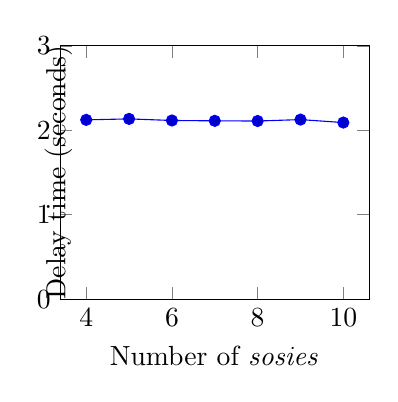
\begin{tikzpicture}
 \begin{axis}[
 	ylabel={Delay time (seconds)},
 	y label style={at={(0.07, 0.5)}}, 	
 	ymin=0,ymax=3,
 	xlabel={Number of \textit{sosies}},width = 5.5cm,
 	height = 4.8cm]

 \addplot+[mark=*] coordinates
 	{(4,2.1235) (5, 2.1348) (6,2.11605) (7,2.1119) (8, 2.1097) (9, 2.12654) (10, 2.09139)};
 	
 \end{axis}
 \end{tikzpicture}
 \caption{\scriptsize Average delay time to detect a faulty \textit{sosie}.\label{fig:delay-time-web-app}}
\end{minipage}
}
\hspace{1cm}
\end{figure}

%	\end{frame}
	
	\subsection[Summary]{Summary}
	
	% DONE - 25
	\begin{frame}{Summary}
		\begin{enumerate}\setlength{\itemsep}{0.7cm}
			\item Lightweight yet efficient monitoring system
				\begin{itemize}
					\item Adaptive monitoring mode that only slowdowns parts of the application
					\item Comparable delay time when a good heuristic is used
				\end{itemize}
			\item Support the definition of application-specific heuristics. In this way developers can:
				\begin{itemize}
					\item Leverages architectural information to drive the search for the
					faulty component
					\item Define Models@runtime-based heuristics
				\end{itemize}
			
			\item Monitoring overhead reduced by 93\%
			
		\end{enumerate}
	\end{frame}
	
	\section{Contributions}
	
	\begin{frame}{Contributions}
		%\framesubtitle{ Synthesis and relation to contributions }
		\begin{scriptsize}
		\begin{block}{\textcolor{gray}{1 -- Scapegoat}}
			\textcolor{gray}{An adaptive resource consumption monitoring framework for component-based systems.}
		\end{block}
		\end{scriptsize}
		%			
		%			\begin{columns}
		%				\column{.57\textwidth}
		%				\begin{itemize}
		%					\item Lack of portable, efficient, and generic resource consumption monitoring tools
		%				\end{itemize}
		%				\column{.01\textwidth}
		%				
		%				\column{.37\textwidth}
		%				\begin{itemize}
		%					\item Scapegoat -- an adaptive monitoring framework
		%				\end{itemize}
		%			\end{columns}
		
		\vspace{0.2cm}
			\begin{block}{{\large 2 -- Squirrel methodology}}
				An architecture-driven approach to reduce the overhead of resource reservation by choosing the proper mapping to represent 
				components in the runtime.
			\end{block}
		\vspace{0.2cm}
		\begin{scriptsize}
			\begin{block}{\textcolor{gray}{3 -- A domain-specific language to define memory profilers}}
				\textcolor{gray}{A generative approach to ease the construction of tools for supporting resource-aware programming. In particular, it support the construction of profilers that can be used at runtime.}
			\end{block}
		\end{scriptsize}
		
		%			\begin{columns}
		%				\column{.47\textwidth}
		%				\begin{itemize}
		%					\item Lack of efficient resource reservation tools for component platforms
		%				\end{itemize}
		%				\column{.01\textwidth}
		%					
		%				\column{.47\textwidth}
		%				\begin{itemize}
		%					\item Squirrel -- an approach to reduce the overhead of resource reservation
		%				\end{itemize}
		%			\end{columns}
		
	\end{frame}
	
	\section[Squirrel -- architecture-driven resource management]{Squirrel -- architecture-driven resource management}
	
	\subsection[Approach]{Approach}
	% DONE - 26
	\begin{frame}{Squirrel -- architecture-driven resource management}
		\textbf{Several approaches to reserve resource}
		\begin{enumerate}[i]
			\item Support different resource types
			\item Impose different overhead 
		\end{enumerate}
		\vspace{1cm}
		\uncover<2>{
			\textbf{What approach to use?}\tikz[remember picture] \node (a) {\vphantom{X}};
			\begin{itemize}
				\item Delay the decision until deployment
				\item Use metadata on architecture to decide
				\item Use extensible component platform supporting:
				\begin{footnotesize}
					\begin{enumerate}[i]
						\item Many mappings from component to system-level abstractions
						\item Each mapping knows how to manage some resource types
					\end{enumerate}
				\end{footnotesize}
				
			\end{itemize}
		}
		\begin{tikzpicture}[remember picture,overlay]
		\path<2> (a.east) ++(3.5,0.7) node[anchor=west,cloud callout,fill=red!50,opacity=.5, callout absolute pointer={(a.mid)}, text width = 2cm]
		{
			\centering{
				\scriptsize
				\underline{Assumption}: \\
				Components do not use resources in the same way.\\[0.8cm]
				\underline{Fact}: \\
				We only know components at deployment time\\
			}
		};
		\end{tikzpicture}
	\end{frame}
	
	% DONE - 27
	\begin{frame}{Squirrel -- Extensible Component Platform}
		\framesubtitle{An implementation to assess the concept}
		\textbf{During component framework design:}
		\begin{enumerate}
			\item Identify mappings from components to system-level abstraction
			\item For each mapping
				\begin{enumerate}[i]
					\item Build resource management mechanisms
					\item Implement optimization for each mechanism
					\item Evaluate mechanisms
					\item Keep the set of most \textit{efficient} mechanisms
				\end{enumerate}
		\end{enumerate}
		\vspace{0.5cm}
		\textbf{At deployment time:}
		\begin{enumerate}
			\item What resources a component requires?
			\item Find the best mapping for each component using multi-objective optimization
			\item Map components to system-level abstraction by wrapping components in resource-aware containers
		\end{enumerate}
	\end{frame}
	
	\subsection[Prototype]{Prototype}
	
	% DONE - 28
	\begin{frame}{An implementation to assess the concept}
		\begin{columns}
			\column{0.5\textwidth}
			\begin{footnotesize}
				\begin{enumerate}
					\item CPU reservation by mapping components to Linux's Cgroups
					\item Memory Reservation using either Scapegoat or isolation components in different JVMs
					\item Optimize communication and deployment time when components are isolated
						\begin{itemize}
							\item Shared-memory channel for communication
							\item Cloning processes to reduce start-up time
						\end{itemize}
				\end{enumerate}
			\end{footnotesize}
			\column{0.5\textwidth}
			\uncover{
				\begin{scriptsize}
					\begin{figure}
						\centering
						\resizebox{0.9\textwidth}{!}{
							%\usetikzlibrary{shadows,arrows}

% Define block styles  
\tikzstyle{cgroup_sty}=[draw, fill=white!20, text width=5em, text centered,
  minimum height=1.4em, rounded corners]

\tikzstyle{thread_sty}=[draw, thin, fill=yellow!20, text width=3em, text centered,
  minimum height=1.4em,dashed]

\tikzstyle{cgroup_container_sty}=[cgroup_sty,fill=gray!20]

\tikzstyle{cgroup_container_hidden_sty}=[cgroup_container_sty,dotted]


\tikzstyle{line} = [draw, thick, color=black!80, -latex']

% commands
\newcommand{\cgroup}[2]{node (p#1) [cgroup_sty]
  {{\scriptsize{#2}}}}

\newcommand{\cgroupContainer}[2]{node (p#1) [cgroup_container_sty]
  {{\scriptsize{#2}}}}

\newcommand{\hiddenCgroup}[2]{node (p#1) [cgroup_container_hidden_sty]
  {{\scriptsize{#2}}}}

\newcommand{\thread}[2]{node (t#1) [thread_sty]
  {{\scriptsize{#2}}}}

\begin{tikzpicture}[scale=0.7,transform shape]
\path \cgroup {1} {Root CGroup};
\path(p1.south) + (-2,-1.2) \cgroupContainer {2} {Cgroup for Kevoree};
\path(p1.south) + (1.7,-1.2) \cgroup {3} {Cgroup for other apps};

\path(p2.south) + (2.3,-1.2) \cgroupContainer {4} {Cgroup for Component2};
\path(p2.south) + (-1.5,-1.6) \cgroupContainer {5} {Cgroup for Component1};

%\path(p4.south) + (0,-1.0) \hiddenCgroup {6} {Hidden Cgroup};
%\path(p5.south) + (0,-1.0) \hiddenCgroup {7} {Hidden Cgroup};

\path [line] (p1) --  node [left] {50\%} (p2);
\path [line] (p1) --  node [right] {50\%} (p3);

\path [line] (p2) --  node [left] {45\%} (p4);
\path [line] (p2) --  node [left] {10\%} (p5);
%\path [line] (p5) --  node [left] {100\%} (p7);
%\path [line] (p4) --  node [right] {100\%} (p6);

\path(p5.south) + (-1.5,-1.2) \thread {1} {Thread1};
\path(p5.south) + (1.8,-1.0) \thread {2} {Thread3};
\path(p5.south) + (0,-1.7) \thread {3} {Thread2};

\path(p4.south) + (0,-1.2) \thread {4} {Thread4};

\path [line] (p5) --  node [above,left] {33\%} (t1);
\path [line] (p5) --  node [above,right] {33\%} (t2);
\path [line] (p5) --  node [left] {33\%} (t3);

\path [line] (p4) --  node [right] {100\%} (t4);

\end{tikzpicture}
						}
						\caption{\scriptsize Reserving CPU by mapping components to cgroups}
					\end{figure}
				\end{scriptsize}
				
			}
		\end{columns}
	\end{frame}
	
	\subsection[Evaluation of the prototype]{Evaluation of the prototype}
	
	% DONE - 29
	\begin{frame}{Research Questions}
		\begin{enumerate}[RQ1]\setlength{\itemsep}{1cm}
			\item What is the impact of the various resource management strategies?
			\item When isolation of component is used as memory management strategy, is the deployment time reduced by using clones of the Kevoree runtime?  
			\item How is communication among components improved by using the proposed optimization?
		\end{enumerate}
	\end{frame}
	
	% DONE - 30
	\begin{frame}{Comparing resource management strategies}
		{} \tikz[remember picture] \node (a) {\vphantom{y}};
		\begin{tikzpicture}[remember picture,overlay]
		\path (a.east) ++(8.7,.2) node[anchor=west,ellipse,fill=red!50,opacity=.5, text width = 2.5cm]
		{
			{\scriptsize
				\centering{\underline{RQ1}}: \\
				What is the impact of the various resource management strategies? \\
			}
		};
		\end{tikzpicture}
		\begin{figure}
			\centering
			\resizebox{0.8\textwidth}{!}{
				\begin{minipage}[t]{0.43\linewidth}
					\centering
					
\pgfplotstableread{
{Test Case}    {Memory Unaware}   {Scapegoat}   {Squirrel} 
xalan	7.910	9.9616	7.957
avrora	10.3672	11.6296	10.3214
batik	1.5054	2.0536	1.3078
fop	0.4774	3.6102	0.4708
luindex	0.7798	1.007	0.6836
lusearch	0.863	6.068	0.935
%pmd	125444	135085	125085
}\data

\begin{tikzpicture}[scale=0.9,transform shape]
  
\begin{axis}[
	every axis legend/.append style={nodes={right}},
	height=4.2cm, width=1\columnwidth,
    ybar=0pt,   % Stacked horizontal bars
    ymin=0,         % Start x axis at 0
    xtick=data,     % Use as many tick labels as y coordinates
    xticklabels from table={\data}{Test Case},  % Get the labels from the Label column of the \datatable
    scaled y ticks = false,
   	y tick label style={
   		/pgf/number format/1000 sep = \thinspace % Optional if you want to replace comma as the 1000 separator 
   	},
    scaled x ticks = false,
   	x tick label style={
   		/pgf/number format/1000 sep = \thinspace % Optional if you want to replace comma as the 1000 separator 
   	},
   	x tick label style={rotate=45},
    bar width = 4,
    ylabel={Execution Time (sec)},
    y label style={at={(0.1,0.5)}},
    legend pos=north west,
    legend style={at={(0.44,0.95)}},
    legend style={font=\tiny},
]
\addplot [fill=white] table [y={Memory Unaware}, x expr=\coordindex] {\data};
\addplot [draw=black,fill=black] table [y={Scapegoat}, x expr=\coordindex] {\data};    % Plot the "First" column against the data index
\addplot [draw=black,pattern=crosshatch] table [y={Squirrel}, x expr=\coordindex] {\data};
\legend{Memory Unaware, Scapegoat, Isolating components}
\end{axis}
\end{tikzpicture}
					\caption{\scriptsize CPU overhead during the execution of Dacapo benchmarks}
				\end{minipage}
				\hspace{0.05\linewidth}
				\begin{minipage}[t]{0.43\linewidth}
					\centering
					
\pgfplotstableread{
{Test Case}    {Memory Unaware}   {Scapegoat}   {Squirrel} 
xalan	30082990.4	393385183.2	53634089.6
avrora	30980142.4	104351584	47699702.4
batik	151662422.4	324599222.4	172317585.6
fop	72838632	756471347.2	97060990.4
luindex	36728345.6	98952945.6	57629534.4
lusearch	23896294.6666667	1182045168	109559376
%pmd	125444	135085	125085
}\data

\begin{tikzpicture}[scale=0.9,transform shape]
  
\begin{axis}[
	every axis legend/.append style={nodes={right}},
	height=4.2cm, width=1\columnwidth,
    ybar=0pt,   % Stacked horizontal bars
    ymin=0,         % Start x axis at 0
    xtick=data,     % Use as many tick labels as y coordinates
    xticklabels from table={\data}{Test Case},  % Get the labels from the Label column of the \datatable
    ytick={268435456,536870912,805306368,1073741824},
    scaled y ticks = false,
   	scaled y ticks=manual:{}{\pgfmathparse{#1/(1024*1024)}},
   	x tick label style={rotate=45},
    bar width = 4,
    ylabel={Memory Usage (MiB)},
    y label style={at={(0.01,0.5)}},
    legend pos=north west,
    legend style={font=\tiny},
]
\addplot [fill=white] table [y={Memory Unaware}, x expr=\coordindex] {\data};
\addplot [draw=black,fill=black] table [y={Scapegoat}, x expr=\coordindex] {\data};    % Plot the "First" column against the data index
\addplot [draw=black,pattern=crosshatch] table [y={Squirrel}, x expr=\coordindex] {\data};
%\legend{Memory Unaware, Scapegoat, Squirrel}
\end{axis}
\end{tikzpicture}
					\caption{\scriptsize Memory overhead during the execution of Dacapo benchmarks}
				\end{minipage}
			}
		\end{figure}
		\centering{
			\color{red} CPU management produces no overhead\\ Memory management produces overhead: Scapegoat is worse
		}
	\end{frame}
	
	% DONE - 31
	\begin{frame}{Importance of optimization for each mapping: \underline{starting time}}
		{} \tikz[remember picture] \node (a) {\vphantom{y}};
		\begin{tikzpicture}[remember picture,overlay]
		\path (a.east) ++(8.7,.6) node[anchor=west,ellipse,fill=red!50,opacity=.5, text width = 2.5cm]
		{
			{\scriptsize
				\centering{\underline{RQ2}}: \\
				When isolation of component is used as memory management strategy, is the deployment time reduced by using clones of the Kevoree runtime? \\
			}
		};
		\end{tikzpicture}
		\begin{figure}
			\centering
			\resizebox{0.85\textwidth}{!}{
				
\pgfplotstableread{
Components    {Processes} {CRIU}   {Plain Kevoree} 
%3        	  547.9745857	2529.407146	155.59293
%4     		  685.5744837	4341.203728	161.0288691
%5       	  743.4672428	5893.812401	171.0221846 
%7       	  1064.555133	9324.145486	162.0639121
%9       	  1268.435203	12563.95009	170.3004435
%12       	  1553.555575	17342.69007	172.6008458
%15 			  2045.492792	22165.56394	192.4309822
3	2.32911218644444	0.790383362555555	0.0907548736666666
4	3.68871036625	1.26219532775	0.12180777075
5	5.15906548553333	1.75811954106667	0.123942168
7	8.10203280628571	2.64415631295238	0.155080078
9	11.3615227505555	3.43788487492592	0.1576709236
12	16.3622474985	5.04937113155556	0.159263136583333
15	21.1857631248444	6.87974225997778	0.1994543878
}\Rapperswil

\begin{tikzpicture}[scale=0.8,transform shape]
  
\begin{axis}[
	every axis legend/.append style={nodes={right}},
	height=4.2cm, width=0.95\columnwidth,
    ybar=0pt,   % Stacked horizontal bars
    ymin=0,         % Start x axis at 0
    xtick=data,     % Use as many tick labels as y coordinates
    xticklabels from table={\Rapperswil}{Components},  % Get the labels from the Label column of the \datatable
    xlabel={Number of components},
    scaled y ticks = false,
%	y tick label style={
%		/pgf/number format/1000 sep = \thinspace % Optional if you want to replace comma as the 1000 separator 
%	},
    scaled x ticks = false,
           x tick label style={
           /pgf/number format/1000 sep = \thinspace % Optional if you want to replace comma as the 1000 separator 
           },
    bar width = 7,
    ylabel={Time (seconds)},
    y label style={at={(0.04, 0.5)}},
    legend pos=north west,
    legend style={font=\tiny},
]
\addplot [fill=white] table [y={Plain Kevoree}, x expr=\coordindex] {\Rapperswil};
\addplot [draw=black,fill=black] table [y=CRIU, x expr=\coordindex] {\Rapperswil};    % Plot the "First" column against the data index
\addplot [draw=black,pattern=crosshatch] table [y=Processes, x expr=\coordindex] {\Rapperswil};
\legend{Plain Kevoree, CRIU, Processes}
\end{axis}
\end{tikzpicture}
			}
			\caption{\scriptsize Average deployment time per component using different strategies}
		\end{figure}
		\centering{
			\color{red} cloning processes reduces starting time overhead from 4000\% to 1900\% 
		}
	\end{frame}
	
	% DONE - 32
	\begin{frame}{Importance of optimizations for each mapping: \underline{communication among isolates}}
		{} \tikz[remember picture] \node (a) {\vphantom{y}};
		\begin{tikzpicture}[remember picture,overlay]
		\path (a.east) ++(8.7,.6) node[anchor=west,ellipse,fill=red!50,opacity=.5, text width = 2.5cm]
		{
			{\scriptsize
				\centering{\underline{RQ3}}: \\
				How is communication among components improved by using the proposed optimizations? \\
			}
		};
		\end{tikzpicture}
		\begin{figure}
			\centering
			\resizebox{.7\textwidth}{!}{
				\begin{minipage}[t]{0.43\textwidth}
					
\pgfplotstableread{
{Data Size}    {NIO}   {Shared Memory}
0	6.298	1.58	
1	6.678	0.92	
1.5849625007	6.27	0.921	
2	6.914	1.012
2.5849625007	6.263	0.909
3	6.92	0.911
3.5849625007	7.14	0.918
3.7004397181	6.678	0.918
4	6.555	0.914
4.2479275134	6.536	0.917
4.3923174228	8.42	0.926
4.5849625007	6.243	0.924
4.7548875022	6.325	0.921
4.8579809951	6.324	0.921
5	6.243	0.915
5.1292830169	8.477	0.917
5.4918530963	7.925	0.925
5.5849625007	7.552	0.915
5.672425342	6.842	0.958
5.9307373376	8.49	0.997
6	8.484	1.199
6.0660891905	8.448	1.083
6.5391588111	8.467	0.946
6.5849625007	6.901	0.922
6.6293566201	8.48	1.104
6.9657842847	8.481	0.932
7	7.184	0.949
}\datatable

%\newcommand\test[1]{
%\pgfmathsetmacro{\var}{#1}
%\pgfmathparse{\varDelta*2} \pgfmathresult}

\definecolor{light-gray}{gray}{0.35}

\begin{tikzpicture}
    \begin{axis}[
    every axis legend/.append style={nodes={right}},
    width= 1\columnwidth,
    height=3.8cm,
    xlabel={Message Size (bytes)},
    ylabel={usec},
    %y label style={pos=east},
    y label style={at={(0.14, 0.5)}},
    x label style={at={(0.5, 0.08)}},
    legend pos=north west,
    legend style={anchor=north west,font=\tiny},
    xtick={0,2,4,6,7},
    %xmode=log,
    %log basis x={2},
    scaled y ticks = false,
    y tick label style={
    	/pgf/number format/1000 sep = \thinspace
    },
    x tick label style={font=\tiny},
    scaled x ticks=manual:{}{%
      	\pgfmathparse{pow(2,#1)}%
    },
    %xticklabel={\pgfmathprintnumber\tick },
    %scaled y ticks=manual:{}{%
    %      	\pgfmathparse{#1/1000}%
    %},
    yticklabel={\pgfmathprintnumber\tick},
    ]
    	\addplot [mark=+,color=black,mark size =1] table[y={Shared Memory}, x = {Data Size}] {\datatable};
    	%\addlegendentry{Shared Memory}[minimum height=1.9in];
    	\addplot [mark=none,color=gray] table[y={NIO}, x ={Data Size}] {\datatable};
    	%\addlegendentry{NIO}[minimum height=1.9in];
    \end{axis}
\end{tikzpicture}
					\vspace{-0.3cm}
					\caption{{\scriptsize Latency of IPC mechanisms}}
				\end{minipage}
				\hspace{0.05\linewidth}
				\begin{minipage}[t]{0.49\textwidth}
					
\pgfplotstableread{
{Data Size}    {Shared Memory}   {NIO} {Named Pipe}
0	4.829262874	1.211303577	2.278292766
1	16.582080532	2.284973183	4.481888576
1.5849625007	24.84903843	3.650475913	7.285710353
2	30.169457071	4.413739735	8.817659304
2.5849625007	50.334063092	7.308872177	12.819947261
3	67.033301105	8.820402778	17.670900556
3.5849625007	99.710387763	12.822872274	25.811055873
3.7004397181	108.088504798	14.851562274	27.280316859
4	133.5675669	18.621127822	35.125028568
4.2479275134	158.098159941	22.179711705	41.054803786
4.3923174228	172.936356172	19.027447421	44.744471279
4.5849625007	198.258407658	29.328904007	51.219885409
4.7548875022	223.640214426	32.568470093	57.679047943
4.8579809951	240.130104691	34.986339417	63.408061398
5	266.9337384	39.106509783	68.524550827
5.1292830169	291.07690972	31.501307665	75.133209088
5.4918530963	371.306741859	43.323522934	95.74922823
5.5849625007	400.371365819	48.490743999	102.375468435
5.672425342	406.104746267	56.872079534	109.795933895
5.9307373376	466.792042028	54.818062952	131.176356948
6	407.150323017	57.550038602	166.253173322
6.0660891905	471.989770733	60.505008949	145.084452028
6.5391588111	749.881978428	83.800438008	219.863148031
6.5849625007	794.093319162	106.139907555	205.538721338
6.6293566201	684.256935216	89.067641012	214.048927819
6.9657842847	1023.734636763	112.453472776	300.145881529
7	1029.584105149	135.930753075	309.12421058
7.0334230015	1027.304169707	116.697242107	285.318100698
7.5622424242	1372.861669051	168.699330324	450.216803756
7.5849625007	1520.213189906	178.617329882	412.373322461
7.6073303137	1487.353476166	223.004631634	414.142278358
7.9829935747	1883.964538087	304.945579899	544.718262454
8	2029.21174905	303.157529871	552.163844844
8.0168082877	2078.834554099	231.545405236	600.765062111
8.5736471875	3004.966139295	424.80696054	984.164634937
8.5849625007	2987.83168967	342.123641214	978.416557876
8.5961897561	2981.563745694	395.555755955	981.559766323
8.9915218461	3955.435559352	611.575583119	1262.459850305
9	3937.062130055	553.18025024	1105.547862345
9.0084286221	3949.038994648	578.762145252	1108.009672612
9.5793159376	5751.338984494	925.793618042	1667.525200127
9.5849625007	5763.6263342	683.90157147	1630.194166837
9.5905870499	5782.042290551	893.794979677	1943.390221041
9.9957671509	7375.253260315	1103.914749616	2555.347488896
10	7420.6583416	1085.280140642	2583.62773537
10.0042204663	7399.879239443	1130.343164423	2545.719136133
10.5821419817	10407.615838242	1528.461298638	3836.099253253
10.5849625007	10459.010591026	1430.78942209	3885.122419844
10.5877775163	10467.367839251	1456.155914263	3378.080700848
10.9978851278	13413.996748093	1803.067395975	4378.763130842
11	13308.791104471	1746.102644706	4540.244522221
11.0021117765	13234.397107891	1994.433990999	5073.758245466
11.5835529305	14022.214827706	3058.174009469	9483.821893006
11.5849625007	17574.180581605	2551.424401063	8084.84927267
11.5863706951	17607.289599655	2533.045417625	8777.943762495
11.9989429514	16565.124813011	4983.721139081	14220.906836006
12	17038.373526088	3774.507385952	12201.364596254
12.0010562746	13210.648128855	4017.979668263	7307.280817184
12.5842578877	23084.476673518	4910.603339731	10086.517395917
12.5849625007	23871.089498227	4966.990490482	9730.990861993
12.5856667697	23709.790397143	5048.779860844	10043.171230086
12.9994715725	29257.910613264	9471.012935496	14228.934368891
13	28683.556655596	6233.173950593	14258.32114591
13.000528234	28549.362950889	7356.552861198	11784.156845751
13.5846102372	34413.107338882	8704.617585743	15821.282060252
13.5849625007	34421.08019242	8713.01377627	16389.392099268
13.5853146782	33561.250799983	10376.784988679	15029.013424612
13.9997358105	25595.465454619	10960.299110444	19477.406159846
14	20223.156583983	10978.068437467	18929.49199111
14.0002641412	25326.378293446	12459.412789012	18114.753416798
14.5847863797	26250.975590243	18111.530868468	23665.630920163
14.5849625007	26235.212219155	15523.929346838	24525.326782535
14.5851386002	25153.809591023	14975.096833361	22628.094517365
14.9998679113	31049.401914693	22139.146166433	26475.952243735
15	31287.197379148	20174.984879434	27180.220598481
15.0001320766	31270.213652828	22299.988561706	25833.004193619
15.5848744429	37764.33788921	24583.590207991	30892.539854137
15.5849625007	35904.006790762	24067.295665602	33595.235558465
15.5850505532	37394.07694005	21385.294903538	30253.574020233
15.9999339572	42024.611702048	22156.773973963	34400.577397926
16	42526.409381948	22768.653369153	33355.416041306
16.0000660398	42135.371754509	22095.615170307	24516.95346759
16.5849184725	46634.977226464	31544.055792361	27346.3375803
16.5849625007	46755.648430194	32020.413157657	27510.498278274
16.5850065276	46622.664838772	28171.132563909	27192.106104393
16.999966979	47238.234258162	29686.823448866	30109.450105664
17	47158.651696736	29563.339750158	29587.405439739
17.0000330203	47199.614834277	29597.736848209	25958.114070443
17.5849404868	45517.942281518	31879.906514408	29219.800949252
17.5849625007	41982.178237447	42632.564123951	29301.331769581
17.5849845143	42661.298716979	31764.349460218	26685.512778575
17.9999834896	46414.692794078	33266.028653703	29164.31928632
18	48395.722679253	33289.438190973	29288.477628167
18.0000165102	47313.280360889	33235.604391119	27216.297460076
18.5849514938	41963.793553975	34805.978837333	28980.488163916
18.5849625007	47278.064642522	34775.082842428	29063.752375911
18.5849735076	48572.455477075	34868.32660189	27847.458660613
18.9999917448	44726.216166649	35271.795693727	28712.569156876
19	43996.571385341	34852.366230723	30321.355537527
19.0000082551	44166.435569925	34783.859418754	27930.63156985
19.5849569973	47809.777463692	34134.247276319	28135.734709709
19.5849625007	50296.361907195	34030.893356802	27890.015515337
19.5849680042	48676.941303384	34022.599544173	27472.353309474
19.9999958724	38427.489532814	32070.098342443	26007.417473416
20	42256.795098438	32078.172520878	25816.481805726
20.0000041276	38698.881552732	38439.343773152	25608.293415362
20.584959749	35059.230140608	33797.506118382	23825.296573269
20.5849625007	35818.974880833	33265.916556813	23229.586947571
20.5849652524	34978.742656498	33338.510640811	23525.150646978
20.9999979362	34120.277968082	36638.090297614	22381.711044179
21	33559.886750483	30035.390170359	22159.744848227
21.0000020638	33559.501904135	36802.61117229	23467.936051512
21.5849611249	33546.715132703	29047.077888273	21312.698704401
21.5849625007	33700.814956603	27241.537806327	20845.600676817
21.5849638766	33590.112667889	25122.081310011	22190.132287542
21.9999989681	34020.557752151	29207.946376923	21985.267189455
22	36599.710799921	26740.547005968	21370.888941467
22.0000010319	33650.321754987	23472.260927074	21320.288845474
22.5849618128	38673.784764138	24061.012240664	21074.406946738
22.5849625007	38397.035748807	24183.159975874	21169.882251247
22.5849631887	38983.24458097	25024.525623474	21033.281053695
22.9999994841	40496.58029954	26704.848945865	21060.137115798
23	39239.62561751	31543.462669175	21287.800372174
23.0000005159	39386.734507184	24765.815374737	21252.918020117
23.5849621568	41827.970702612	24697.332265871	21202.259955687
23.5849625007	40619.018086321	24819.606183673	21210.578420379
23.5849628447	41555.364882277	24693.315933731	21239.175518618
23.999999742	44010.813883148	25069.671590142	21516.756380553
24	40511.402959623	30577.659465717	21338.137123936
24.000000258	44163.081035384	24941.099097069	21130.768793943
24.5849623287	45012.376923834	31862.436201921	21028.171829476
24.5849625007	44953.407171271	28507.061514714	21051.65818326
24.5849626727	44935.723920206	27605.865978166	21537.009044472
24.999999871	44319.700398091	26207.879591305	21504.783088481
25	45073.569333923	25473.326348502	21218.921527418
25.000000129	44989.096064651	25261.482217836	21405.021012988
25.5849624147	45467.797522632	30801.895171737	21235.367941674
25.5849625007	46262.358425389	25250.400756266	21143.089769114
25.5849625867	46150.097961305	25250.152249501	21619.956304471
25.9999999355	46457.977161832	25235.946710162	23090.944124277
26	45875.905187715	25306.504292221	21292.597742437
26.0000000645	46107.020585404	25344.246828366	21461.749130172
}\datatable

\definecolor{light-gray}{gray}{0.35}

\begin{tikzpicture}
    \begin{axis}[
    every axis legend/.append style={nodes={right}},
    width= 1\columnwidth,
    height=3.8cm,
    xlabel={Message Size (bytes)},
    ylabel={Gbps},
    %y label style={pos=east},
    y label style={at={(0.1, 0.5)}},
    x label style={at={(0.5, 0.08)}},
    legend pos=north west,
    legend style={anchor=north west,font=\tiny},
    xtick={0,4,8,12,16,20,24,26},
    %xmode=log,
    %log basis x={2},
    scaled y ticks = false,
    y tick label style={
    	/pgf/number format/1000 sep = \thinspace
    },
    x tick label style={font=\tiny},
    xtick={0,4,8,12,16,20,24},
    xticklabels={
      1,16,256,4\,Kb,64\,Kb,1\,Mb,16\,Mb
    },
    scaled y ticks=manual:{}{%
          	\pgfmathparse{#1/1000}%
    },
    yticklabel={\pgfmathprintnumber\tick},
    ]
    	\addplot [mark=+,mark size =1,color=black] table[y={Shared Memory}, x = {Data Size}] {\datatable};
    	\addlegendentry{Shared Memory}[minimum height=1.9in];
    	\addplot [mark=none,color=gray] table[y={NIO}, x ={Data Size}] {\datatable};
    	\addlegendentry{NIO}[minimum height=1.9in];
    	%\addplot [mark=*,mark size =0.5,color=blue] table[y={Named Pipe}, x ={Data Size}] {\datatable};
    	%\addlegendentry{Named Pipe}[minimum height=1.9in];
    \end{axis}
\end{tikzpicture}
					\vspace{-0.3cm}
					\caption{{\scriptsize Bandwidth of IPC mechanisms}}
				\end{minipage}
			}
		\end{figure}
		\vspace{-0.5cm}
		\begin{figure}
			\centering
			\resizebox{0.55\textwidth}{!}{
				
\pgfplotstableread{
{Components}   {NIO+Builtin} {NIO+FST} {Shared Memory+Builtin} {Shared Memory+FST}
1	9.5757382966045	21.5430618770379	9.7620268732395	25.9297426880135
2	7.6422174248457	17.5126876795335	7.5310355481145	21.0667494056227
3	5.250704274339	12.9178921978644	6.0802882854381	16.15260490071
4	4.3413147942753	10.0750437619601	4.5948850025035	11.7925202756171
5	3.4491399072965	8.539957899374	3.6971062586641	10.2725891101392
6	2.7280490283444	7.0238142280927	3.0884059889541	7.92238942117
7	2.3306217714334	5.6761283469114	2.7639583086961	7.0266894534711
8	2.0645411102461	5.2233197450063	2.3809104485843	5.9730099510704
}\Rapperswil

\begin{tikzpicture}
    \begin{axis}[
    every axis legend/.append style={nodes={right}},
    width=0.9\columnwidth,
    height=4.0cm,
    x tick label style={/pgf/number format/1000 sep=},
    xlabel={Consumers},
    ylabel={k msg/sec},
    y label style={at={(0.05, 0.5)}},
	scaled y ticks = false,
%	y tick label style={
%	    	/pgf/number format/1000 sep = \thinspace
%	},
	%legend pos=north west,
    legend style={anchor=north west,font=\tiny},
    legend style={at={(0.55,0.95)}},
    legend columns=1,
    %legend style={text width=1.8cm}
    mark size=1.5
    ]
    \addplot [mark=+, color = black] table[y={Shared Memory+FST}, x={Components}] {\Rapperswil};
    \addlegendentry{Shared Memory+FST};
    \addplot [mark=*, color= gray] table[y={NIO+FST}, x={Components}] {\Rapperswil};
    \addlegendentry{NIO+FST};
    \addplot[mark=*, color = black] table[y={Shared Memory+Builtin}, x={Components}] {\Rapperswil};
    \addlegendentry{Shared Memory+Builtin}[minimum height=1.9in];    	    
    \addplot [mark=none, color = gray] table[y={NIO+Builtin}, x={Components}] {\Rapperswil};
    \addlegendentry{NIO+Builtin};	
    \end{axis}
\end{tikzpicture}
			}
			\vspace{-0.5cm}
			\caption{{\tiny Communication throughput for different channels}}
		\end{figure}
		\vspace{-.3cm}
		\centering{\color{red} Proper channels reduce the cost of isolation in terms of communications}
	\end{frame}
	
	\subsection[Summary]{Summary}
	
	% DONE - 33
	\begin{frame}{Summary}
		\begin{itemize}\setlength{\itemsep}{1cm}
			\item A late binding approach to reduce the cost of resource management
			\item A prototype implemented using the Kevoree component framework
				\vspace{0.5cm}
				\begin{itemize}\setlength{\itemsep}{0.5cm}
					\item Different mapping for components
					\item Different optimization strategies
				\end{itemize}
		\end{itemize}
		\vfill
	\end{frame}
	

\newcommand{\kw}[1]{\textbf{\color{blue} #1}}

	\section{Contributions}

	\begin{frame}{Contributions}
		%\framesubtitle{ Synthesis and relation to contributions }
		\begin{scriptsize}
			\begin{block}{\textcolor{gray}{1 -- Scapegoat}}
				\textcolor{gray}{An adaptive resource consumption monitoring framework for component-based systems.}
			\end{block}
			\begin{block}{\textcolor{gray}{2 -- Squirrel methodology}}
				\textcolor{gray}{An architecture-driven approach to reduce the overhead of resource reservation by choosing the proper mapping to represent components in the runtime.}
			\end{block}
		\end{scriptsize}
		%			
		%			\begin{columns}
		%				\column{.57\textwidth}
		%				\begin{itemize}
		%					\item Lack of portable, efficient, and generic resource consumption monitoring tools
		%				\end{itemize}
		%				\column{.01\textwidth}
		%				
		%				\column{.37\textwidth}
		%				\begin{itemize}
		%					\item Scapegoat -- an adaptive monitoring framework
		%				\end{itemize}
		%			\end{columns}
		
		
		\vspace{0.2cm}
		\begin{block}{{\large 3 -- A domain-specific language to define memory profilers}}
			A generative approach to ease the construction of tools for supporting resource-aware programming. In particular, it support the construction of profilers that can be used at runtime.
		\end{block}
		
		%			\begin{columns}
		%				\column{.47\textwidth}
		%				\begin{itemize}
		%					\item Lack of efficient resource reservation tools for component platforms
		%				\end{itemize}
		%				\column{.01\textwidth}
		%					
		%				\column{.47\textwidth}
		%				\begin{itemize}
		%					\item Squirrel -- an approach to reduce the overhead of resource reservation
		%				\end{itemize}
		%			\end{columns}
		
	\end{frame}

	\section{Building efficient domain-specific memory profilers}
	
	% DONE 
	\begin{frame}{Customized memory profilers}
		\textbf{Software abstractions are at the core of development}
		\begin{enumerate}[i]
			\item Components, Domain-Specific Languages
			\item Development tools lack support for new abstractions
			\item Time consuming writing them from scratch 
		\end{enumerate}
		\vspace{1cm}
		\uncover<2>{
			\textbf{Generative approach to the rescue}\tikz[remember picture] \node (a) {\vphantom{X}};
			\begin{itemize}
				\item Backend technology to perform the actual profiling
				\item What kind of information we want to compute?
				\item How we represent the great diversity of abstractions?				
			\end{itemize}
		}
		\begin{tikzpicture}[remember picture,overlay]
		\path<2> (a.east) ++(3.0,0.7) node[anchor=west,cloud callout,fill=red!50,opacity=.5, callout absolute pointer={(a.east)}, text width = 2cm]
		{
			\centering{
				\scriptsize
				\underline{Observation}: \\
				In a MRTE all abstractions are represented by objects in memory\\ 
			}
		};
		\end{tikzpicture}
	\end{frame}
	
	\subsection[Motivating Examples]{Motivating Examples}
	% DONE
	\begin{frame}{Number of objects reachable from a given object}
		\begin{figure}[!ht]
			\centering
			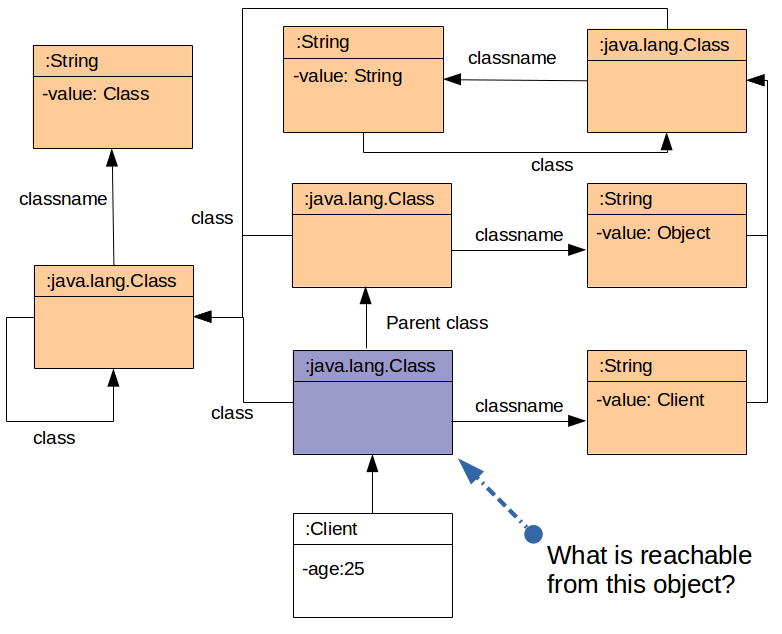
\includegraphics[scale=0.3]{../chapter6/fig/example1.png}
			\caption{\scriptsize Objects reachable from the Client class. Observe that only one object is not reachable.}
		\end{figure}
		\centering{
			\color{red} This is a \underline{graph}, and we are \underline{computing values} in a \underline{subgraph}
		}
	\end{frame}
	
	% DONE
	\begin{frame}{Length of singly linked lists}
		\begin{figure}[!ht]
			\centering
			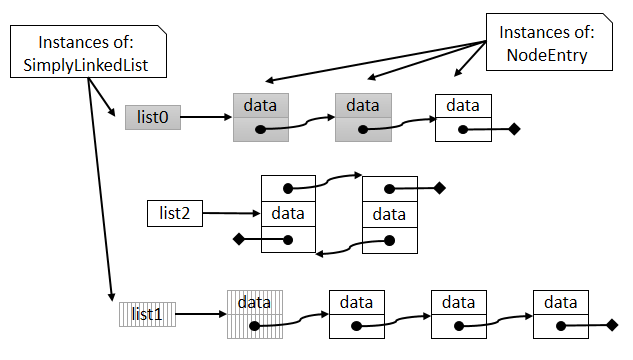
\includegraphics[scale=0.3]{../chapter6/fig/lists}
			\vspace{-.3cm}
			\caption{\scriptsize Memory snapshot with three linked lists}
		\end{figure}
		%\vspace*{-0.1cm}
		{\footnotesize
		\begin{equation*}
			f_{\textit{head}}\left(O\right) = 
			\begin{cases}
			\textit{head} = O & \quad O \; is \; \operatorname{SinglyLinkedList} \\
			\exists {x \in \operatorname{Objects}}, \quad x \operatorname{references} o \wedge f_{\textit{head}}\left(x\right) & \quad O \; is \; \operatorname{NodeEntry} \\
			\operatorname{false} & \quad \operatorname{otherwise} \\
			\end{cases}
		\end{equation*}
		}
		\vspace{0.2cm}
		\begin{alertblock}{Other subgraphs (there are many lists)}
			A recursive equation determines whether an object is member of a subgraph
		\end{alertblock}
	\end{frame}
	
	\subsection[Approach]{Approach}
	
	% DONE
	\begin{frame}{Idea for a domain-specific language to define memory profilers}
		\begin{enumerate}
			\item An instance of a software abstraction is represented as a collection of objects at runtime -- a subgraph
			\item We call such subgraphs \underline{\textbf{structures}}
			\item The idea is to identify structures and to compute values on them.
			\begin{itemize}
				\item Size
				\item Number of Objects
				\item How many objects in the structure met a first order predicate
			\end{itemize}
		\end{enumerate}
		\vfill
		\begin{alertblock}{The garbage collector knows how to traverse the whole graph -- linear time}
			\begin{enumerate}[S1]
				\item For each object, checks if it is member of a \textit{\textbf{structure}}
				\item If \textit{yes}, perform a partial computation of the value associated to such a \textit{\textbf{structure}}
			\end{enumerate}
		\end{alertblock}
		
		%{
		%	\centering{\color{red} Our goal is to identify the structures in linear time with respect to the number of objects in the heap }\\
		%	\centering{\scriptsize \underline{}}\\
		%}
	\end{frame}
	
	\begin{frame}{Global Architecture}
		\begin{figure}[!ht]
			\centering
			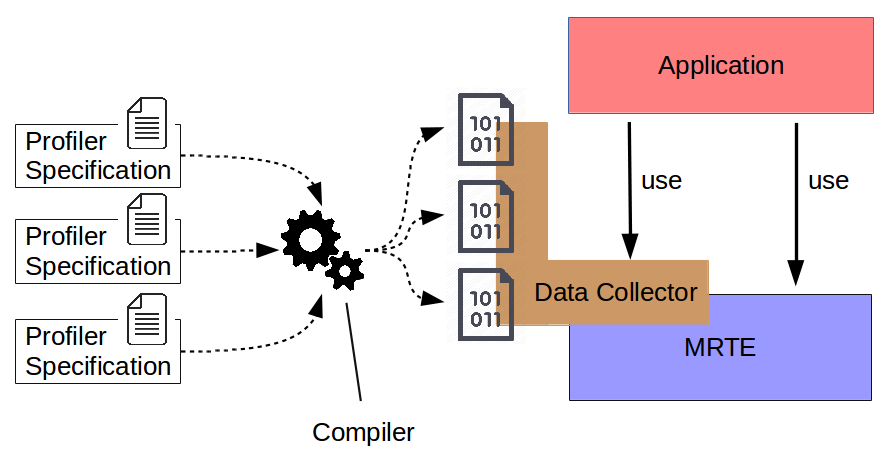
\includegraphics[scale=0.3]{../chapter6/fig/global-view.png}
			\caption{\scriptsize In this case, three memory profilers are defined.}
		\end{figure}
	\end{frame}
	
	\begin{frame}{Declaring Types For Collecting Data}
		\begin{block}{Concrete Syntax}
			\hspace{1cm} \textcolor{red}{\textbf{Type}} ::= \textcolor{red}{\textbf{id}} `\textcolor{Emerald}{:}' (`\textcolor{Emerald}{tableOf}' \textcolor{red}{\textbf{id}} $|$ `\textcolor{Emerald}{struct}' `\textcolor{Emerald}{\{}' (\textcolor{red}{\textbf{id}} `\textcolor{Emerald}{:}' \textcolor{red}{\textbf{id}})$+$  `\textcolor{Emerald}{\}}') 
		\end{block}
		\begin{columns}
			\column{0.48\textwidth}
			\begin{exampleblock}<2->{Structures}
				\begin{footnotesize}
					\hspace{.3cm} \textcolor{Emerald}{// A simple structure} \\
					\hspace{.3cm} WantedObject : \kw{struct} \{ \\
					\hspace{.6cm} class\_name : \textbf{string} \\
					\hspace{.6cm} size : \textbf{int} \\
					\hspace{.3cm} \} \\
				\end{footnotesize}
			\end{exampleblock}
			\column{0.48\textwidth}
			\begin{exampleblock}<3->{Tables}
				\begin{footnotesize}
					\hspace{.3cm} \textcolor{Emerald}{// This new type is a table (i.e., list)} \\
					\hspace{.3cm} \textcolor{Emerald}{// of WantedObject} \\
					\hspace{.3cm} wanted : \kw{tableOf} WantedObject \\
					\hspace{.3cm} \textcolor{Emerald}{// In the language, values of this type} \\
					\hspace{.3cm} \textcolor{Emerald}{// have operations such as \textit{map} and \textit{filter}} \\
				\end{footnotesize}
			\end{exampleblock}
		\end{columns}
		\begin{columns}
			\centering
			\column{0.4\textwidth}
			\begin{block}<4->{Built-In Types}
				\begin{itemize}
					\item \textbf{int}
					\item \textbf{bool}
					\item \textbf{string}
				\end{itemize}
			\end{block}
		\end{columns}
	\end{frame}
	
	\begin{frame}{Expressions}
		\begin{columns}
			\column{0.4\textwidth}
			\begin{exampleblock}<1->{Basic}
				\begin{footnotesize}
					\hspace{.1cm} \textcolor{Emerald}{// simple arithmetic} \\
					\hspace{.1cm} 3 + i \\
					\hspace{.1cm} \textcolor{Emerald}{// boolean operators} \\
					\hspace{.1cm} flag \kw{and} (12 $>$ a) \\
					\hspace{.1cm} \textcolor{Emerald}{// string to int} \\
					\hspace{.1cm} \textcolor{NavyBlue}{``12''}.toInt() + 4 \\
					\hspace{.1cm} 12.toString() \textcolor{Emerald}{// int to string}\\
				\end{footnotesize}
			\end{exampleblock}
			\column{0.56\textwidth}
			\begin{exampleblock}<2->{Initializing structures and tables}
				\begin{footnotesize}
					\hspace{.1cm} \textcolor{Emerald}{ // a table value that contains 1, 2, 3} \\
					\hspace{.1cm} \#[ 1,2,3 ] \\
					\hspace{.1cm} \textcolor{Emerald}{// a structure value WantedObject} \\
					\hspace{.1cm} \kw{struct} WantedObject \{ \textcolor{NavyBlue}{``String''}, \textit{12 + 3} \} \\
					\hspace{.1cm} \textcolor{Emerald}{// a list of WantedObject with one element} \\
					\hspace{.1cm} \#[ \kw{struct} WantedObject \{ \textcolor{NavyBlue}{``Integer''}, i*4 \} ]\\ % \textcolor{Emerald}{// one element} \\
					\hspace{.1cm} \textcolor{Emerald}{// an empty list of string} \\
					\hspace{.1cm} \#\textbf{string}[] \textcolor{Emerald}{// need the type qualifier } \\
				\end{footnotesize}
			\end{exampleblock}
		\end{columns}
		\vspace{0.3cm}
		\begin{columns}
			\centering
			\column{0.9\textwidth}
			\begin{exampleblock}<3->{Lambda Expressions}
				\begin{footnotesize}
					\hspace{.1cm} \textcolor{NavyBlue}{// keep three in the result} \\
					\hspace{.1cm} \#[ 1,2,3 ].filter([it $|$ it $>$ 2])
					\hspace{.1cm} {}\\
					\hspace{.1cm} \textcolor{NavyBlue}{// instances of class K3Object} \\
					\hspace{.1cm} \underline{objects}.filter([it $|$ it \kw{is} K3Object]) \textcolor{NavyBlue}{// \textit{objects is a built-in value}}\\
					\hspace{.1cm} \textcolor{NavyBlue}{// keep metadata of ``big'' objects } \\
					\hspace{.1cm} \underline{objects}.filter([it $|$ it $>$ 1000]).map([it $|$ \kw{struct} WantedObject \{ it.\underline{classname}, it.\underline{size} \}]) \\
				\end{footnotesize}
			\end{exampleblock}
		\end{columns}
	\end{frame}
	
	\begin{frame}{Defining structures in the heap}
		\begin{block}{Concrete Syntax}
			\hspace{1cm} \textcolor{red}{\textbf{structure}} ::= `\textcolor{Emerald}{create structure foreach}' \textcolor{red}{\textbf{id}} `\textcolor{Emerald}{:}' \textcolor{red}{\textbf{exp}} `\textcolor{Emerald}{using}' \textcolor{red}{\textbf{body}} \\ 
			\hspace{1cm} \textcolor{red}{\textbf{body}} ::= `\textcolor{Emerald}{constructor}' \textcolor{red}{\textbf{stmts}} `\textcolor{Emerald}{membership}' \textcolor{red}{\textbf{exp}} `\textcolor{Emerald}{updates}' \textcolor{red}{\textbf{stmts}} \\
			\hspace{1cm} \textcolor{red}{\textbf{stmts}} ::= (\textcolor{red}{\textbf{id}} `\textcolor{Emerald}{=}' \textcolor{red}{\textbf{exp}} ) $+$\\
		\end{block}
		\begin{columns}
			\column{0.6\textwidth}
			\begin{exampleblock}<1->{Number of instances of two classes}
				\begin{footnotesize}
					\hspace{.1cm} \kw{create structure foreach} e:\#[\textcolor{NavyBlue}{``JFrame''}] \kw{using} \\
					\hspace{.3cm} \kw{constructor} \\
					\hspace{.5cm} \textbf{\textit{initialObjects}} = \#Object[] \textcolor{Emerald}{// built-in value} \\
					\hspace{.5cm} n = 0 \textcolor{Emerald}{// compute value n in this structure} \\
					\hspace{.3cm} \kw{membership} \kw{\textit{this}} \kw{is} JFrame \textcolor{Emerald}{// \textit{this} is built-in value} \\
					\hspace{.3cm} \kw{updates} n = n + 1 \\
					\vspace{0.2cm}
					\hspace{.1cm} \textcolor{Emerald}{// defining another type of structure } \\
					\hspace{.1cm} \kw{create structure foreach} e:\#[\textcolor{NavyBlue}{``JPane''}] \kw{using} \\
					\hspace{.3cm} \kw{constructor} \\
					\hspace{.5cm} \textbf{\textit{initialObjects}} = \#Object[] \\
					\hspace{.5cm} m = 0 \\
					\hspace{.3cm} \kw{membership} \kw{\textit{this}} \kw{is} JPane \\
					\hspace{.3cm} \kw{updates} m = m + 1 \\
				\end{footnotesize}
			\end{exampleblock}
		\end{columns}
	\end{frame}
	
	%\begin{frame}{Abstract Syntax}
	%	\begin{figure}
	%		\centering
	%		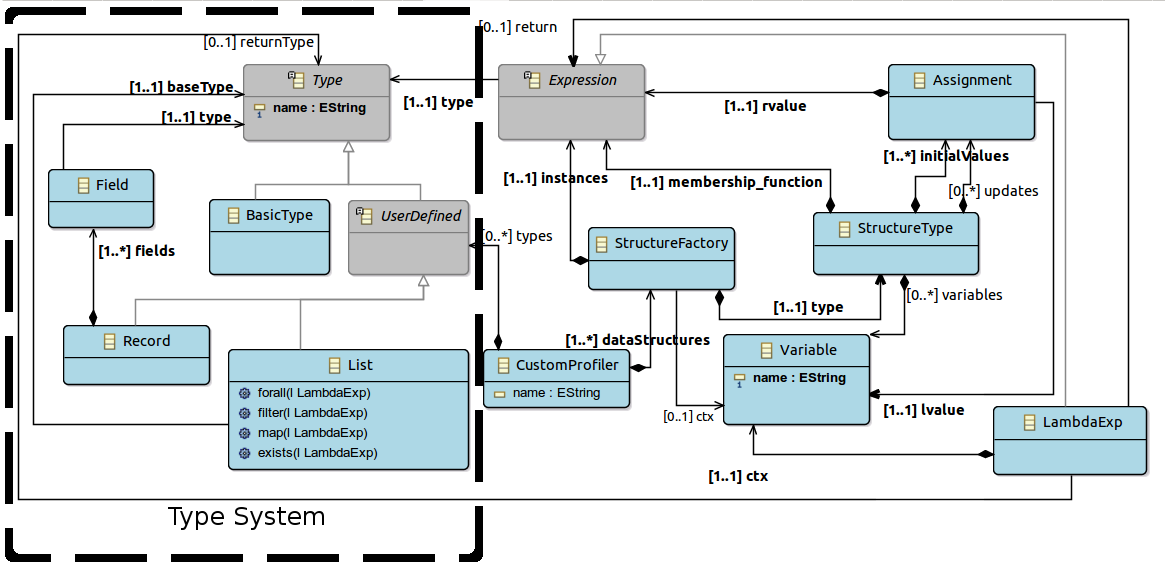
\includegraphics[width=0.93\linewidth]{../chapter6/fig/AS}
	%		\caption{\scriptsize Meta-model for representing customized memory profilers}
	%	\end{figure}
	%\end{frame}
	
	\begin{frame}{Developers View}
		\begin{columns}
			\column{0.65\textwidth}
			\begin{block}{Create software abstraction for other developers}
				\begin{scriptsize}
					\begin{itemize}
						\item Component framework
						\item Library for a given domain
						\item Domain-specific language
					\end{itemize}
				\end{scriptsize}
			\end{block}
			\column{0.28\textwidth}
		\end{columns}
		\begin{columns}
			\column{0.25\textwidth}
			\begin{block}{Deliver software}
				\begin{scriptsize}
					Include domain-specific memory profilers along the \textit{software abstraction} to ease its usage.
				\end{scriptsize}
			\end{block}
			
			\begin{alertblock}{Native agent}
				\begin{scriptsize}
					JVMTI is used to traverse the graph of objects\\
				\end{scriptsize}
			\end{alertblock}
			\column{0.65\textwidth}
			
			\begin{figure}
				\hfill
				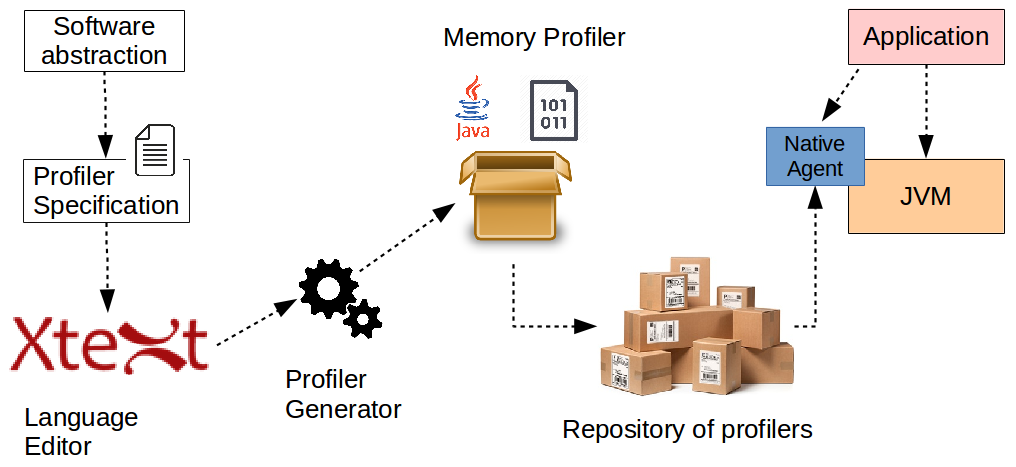
\includegraphics[scale=0.3]{../chapter6/fig/developer-profiler-view.png}
				\vspace{-.3cm}
				\caption{\scriptsize Memory profilers are built from the description of software abstractions}
			\end{figure}
		\end{columns}
	\end{frame}
	
	\begin{frame}{Users View}
		\begin{columns}
			\column{0.70\textwidth}
			\begin{figure}
				\centering
				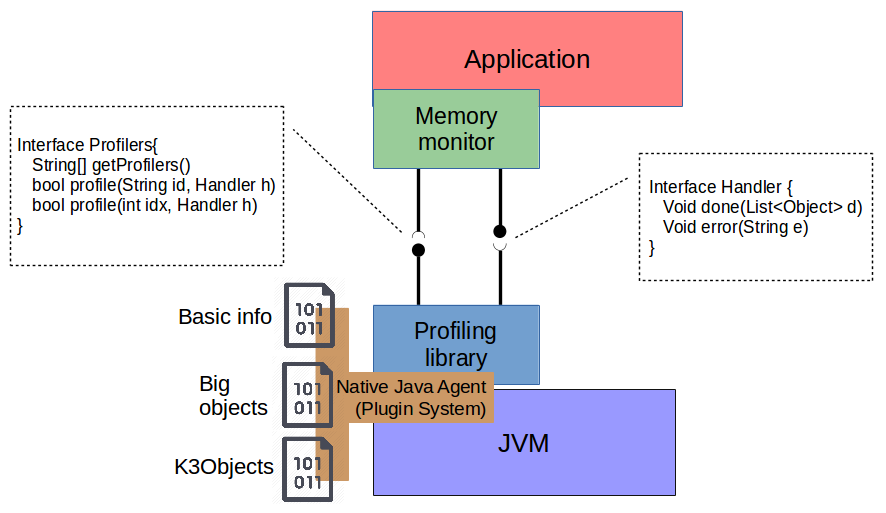
\includegraphics[scale=0.35]{../chapter6/fig/user-profiler-view.png}
				%\caption{\scriptsize . Data collected is in the form of plain Java objects.}
			\end{figure}
			\column{0.25\textwidth}
		\end{columns}
		\vspace{.3cm}
		\begin{columns}
			\column{0.25\textwidth}
			\column{0.65\textwidth}
			\begin{alertblock}{Accessing profilers}
				\begin{scriptsize}
					\begin{itemize}
						\item Memory profilers are black-boxes accessed through Java interfaces
						\item Data is collected in the form of plain Java objects
					\end{itemize}
				\end{scriptsize}
			\end{alertblock}
		\end{columns}
	\end{frame}
	
	\subsection[Evaluation]{Evaluation}
	
	% DONE 
	\begin{frame}{Research Questions}
		\begin{enumerate}[RQ1]\setlength{\itemsep}{1cm}
			\item Is significant the difference between the time needed to execute a single analysis with our approach in comparison to previous solutions?  
			\item Does our approach produce profilers with lower overhead than state-of-the-art tools when used to perform many iterations of memory analysis at runtime?
			\item Does the advantages of our approach remain for real applications?
		\end{enumerate}
	\end{frame}
	
	\begin{frame}{Analysis Time}
		{} \tikz[remember picture] \node (a) {\vphantom{y}};
		\vspace{-.5cm}
		\begin{scriptsize}
			\begin{example}
				\hspace{.3cm} \kw{create structure foreach} e:\#["jvm"], \kw{using}\\
				\hspace{.6cm} \kw{constructor} \\
				\hspace{.9cm} initialObjects = \#[Object] \\
				\hspace{.9cm} exists = false \\
				\hspace{.6cm} \kw{membership}  true \\
				\hspace{.6cm} \kw{updates} exists = exists \kw{or} (this \kw{is} UnusedClass) \\
			\end{example}
		\end{scriptsize}
		\begin{tikzpicture}[remember picture,overlay]
		\path (a.east) ++(8.7,.0) node[anchor=west,ellipse,fill=red!50,opacity=.5, text width = 2.5cm]
		{
			{\scriptsize
				\centering{\underline{RQ1}}: \\
				Is significant the difference between the time needed to execute a single analysis with our approach in comparison to previous solutions? \\
			}
		};
		\end{tikzpicture}
		\vspace{-.4cm}
		\begin{figure}[!ht]
 \centering
\resizebox{.8\textwidth}{!}{
 \begin{minipage}[t]{0.45\linewidth}
 \centering
\begin{tikzpicture}
\begin{axis}[
ybar=0pt, 
legend style={at={(0.72,1)},
every axis legend/.append style={nodes={right}},
anchor=north,legend columns=1, font=\tiny},
ylabel={Analysis Time (sec)},
y label style={at={(0.1, 0.5)}},
scaled y ticks = false,
      y tick label style={/pgf/number format/fixed, font=\scriptsize,
      /pgf/number format/1000 sep = \thinspace % Optional if you want to replace comma as the 1000 separator 
      },
xtick=data,ymin=0,
width = \columnwidth,
height = 4.0cm,
bar width = 4,
x tick label style={rotate=45,anchor=east, font=\scriptsize},
 axis lines*=left, % Don't display the top and right lines
 symbolic x coords={antlr,fop,hsqldb,jython,chart,luindex,xalan,lusearch, pmd, eclipse}
]
\addplot coordinates 
	{(antlr,1.9781514264) (fop,1.605707750) (hsqldb,2.2388250106) (jython,1.3401924419) (chart,2.9126870659) (luindex,1.4126736676)
	(xalan,1.5175679043) (lusearch,2.1071653048) (pmd,1.1071653048) (eclipse,3.2922104461) };
\addplot coordinates 
	{(antlr,2.2781514264) (fop,1.805707750) (hsqldb,2.5388250106) (jython,1.6401924419) (chart,3.2126870659) (luindex,1.6126736676)
		(xalan,1.7175679043) (lusearch,2.4071653048) (pmd,1.3071653048) (eclipse,3.5922104461) };
\addplot coordinates 
	{(antlr,2.9781514264) (fop,2.605707750) (hsqldb,3.2388250106) (jython,2.3401924419) (chart,3.9126870659) (luindex,2.4126736676)
		(xalan,2.5175679043) (lusearch,3.1071653048) (pmd,2.1071653048) (eclipse,4.2922104461) };
%\legend{Handwritten JVMTI, Our approach, Heap Dump + Eclipse MAT}
\end{axis}
\end{tikzpicture}
\vspace{-.3cm}
\caption{\scriptsize Analysis time with default input size}
\end{minipage}
\hspace{0.03\linewidth}
\begin{minipage}[t]{0.45\linewidth}
 \centering
\begin{tikzpicture}
\begin{axis}[ybar=0pt, legend style={at={(1.08,1.23)},
every axis legend/.append style={nodes={right}},
anchor=north,legend columns=1, font=\tiny},
ylabel={Analysis Time (sec)},
y label style={at={(0.1, 0.5)}},
scaled y ticks = false,
      y tick label style={/pgf/number format/fixed, font=\scriptsize,
      /pgf/number format/1000 sep = \thinspace % Optional if you want to replace comma as the 1000 separator 
      },
xtick=data,ymin=0,
width = \columnwidth,
height = 4.0cm,
bar width = 4,
x tick label style={rotate=45,anchor=east, font=\scriptsize},
 axis lines*=left, % Don't display the top and right lines
 symbolic x coords={antlr,fop,hsqldb,jython,chart,luindex,xalan,lusearch, pmd, eclipse}
]
\addplot coordinates 
	{(antlr,2.3781514264) (fop,1.905707750) (hsqldb,2.7388250106) (jython,1.8401924419) (chart,3.1126870659) (luindex,1.6126736676)
	(xalan,1.7175679043) (lusearch,2.2171653048) (pmd,1.3171653048) (eclipse,3.3822104461) };
\addplot coordinates 
	{(antlr,2.5781514264) (fop,1.945707750) (hsqldb, 2.7818250106) (jython,2.0401924419) (chart,3.6326870659) (luindex,1.912632376)
		(xalan,1.9375679043) (lusearch,2.4071653048) (pmd,1.3999716530) (eclipse,3.7922104461) };
\addplot coordinates 
	{(antlr,3.9781514264) (fop,3.605707750) (hsqldb,4.2388250106) (jython,3.3401924419) (chart,4.9126870659) (luindex,3.4126736676)
		(xalan,3.5175679043) (lusearch,4.1071653048) (pmd,3.1071653048) (eclipse,5.2922104461) };
\legend{Handwritten JVMTI, \underline{Our approach}, \underline{Heap Dump + Eclipse MAT}}
\end{axis}
\end{tikzpicture}
\vspace{-.3cm}
\caption{\scriptsize Analysis time with large input size}
 \end{minipage}
}
\end{figure}

		\vspace{-.3cm}
		\begin{columns}
			\column{0.5\textwidth}
			\centering{\color{red} \underline{Analysis time reduced between 25\% and 39\%}}
			\column{0.5\textwidth}
			\centering{\color{red} 150+ sloc in handwritten solution \\ 3+ sloc in Eclipse MAT}
		\end{columns}
	\end{frame}

	\begin{frame}{Total Execution Time}
		{} \tikz[remember picture] \node (a) {\vphantom{y}};
		\vspace{-0.7cm}
		\begin{scriptsize}
			\begin{example}
				\hspace{.3cm} Info : \kw{struct} \{ nbObjects : int, size : int \} \\
				\hspace{.3cm}	\kw{create structure foreach} e:\#["whole-jvm"] \kw{using} \\
				\hspace{.6cm}	\kw{constructor} \\
				\hspace{.9cm}	initialObjects = threads \\
				\hspace{.9cm}	data = \kw{struct} Info \{ 0, 0 \} \\
				\hspace{.6cm}	\kw{membership} ( referrer \kw{in} this\_structure ) \\
				\hspace{.6cm}	\kw{updates} \\
				\hspace{.9cm}	data = \kw{struct} Info \{ data.nbObjects + 1 , data.size + this.size \}
			\end{example}
		\end{scriptsize}
		\begin{tikzpicture}[remember picture,overlay]
		\path (a.east) ++(8.7,.3) node[anchor=west,ellipse,fill=red!50,opacity=.5, text width = 2.5cm]
		{
			{\scriptsize
				\centering{\underline{RQ2}}: \\
				Does our approach produce profilers with lower overhead than state-of-the-art tools when used to perform many iterations of memory analysis at runtime? \\
			}
		};
		\end{tikzpicture}
		\vspace{-.4cm}
		\begin{figure}[!ht]
\centering
\resizebox{.8\textwidth}{!}{
\begin{tikzpicture}
\begin{axis}[ybar=0pt, legend style={at={(0.72,1)},
every axis legend/.append style={nodes={right}},
anchor=north,legend columns=1, font=\tiny},
ylabel={Overhead (\%)},
y label style={at={(0.02, 0.5)}},
scaled y ticks = false,
      y tick label style={/pgf/number format/fixed, font=\scriptsize,
      /pgf/number format/1000 sep = \thinspace % Optional if you want to replace comma as the 1000 separator 
      },
xtick=data,ymin=0,
width = 0.9\columnwidth,
height = 3.5cm,
bar width = 7,
x tick label style={rotate=45,anchor=east,font=\scriptsize},
 axis lines*=left, % Don't display the top and right lines
 symbolic x coords={antlr,fop,hsqldb,jython,chart,luindex,xalan,lusearch, pmd, eclipse}
]
\addplot coordinates 
	{(antlr,3.9781514264) (fop,4.605707750) (hsqldb,29.2388250106) (jython,1.3401924419) (chart,2.9126870659) (luindex,7.4126736676)
	(xalan,3.5175679043) (lusearch,2.1071653048) (pmd,2.1071653048) (eclipse,13.2922104461) };
\addplot coordinates 
	{(antlr,4.6792415918) (fop,10.920169369) (hsqldb,33.4078193658) (jython,7.3669103815) (chart,10.0961181121) (luindex,5.8949045922) 
	(xalan,10.6595492114) (lusearch,8.8185623499) (pmd,11.7847827707) (eclipse,15.7219232736)};
\addplot coordinates 
	{(antlr,28.7859273871) (fop,23.7271506764) (hsqldb,46.0448750552) (jython,32.4395399802) (chart,44.6349538836) (luindex,31.9874187461) 
	(xalan,37.7533619117) (lusearch,12.9664891096) (pmd,33.9112866499) (eclipse,32.6863711858)};
\legend{Handwritten JVMTI, \underline{Our approach}, Heap Dump + Eclipse MAT}
\end{axis}
\end{tikzpicture}
}
\vspace{-.5cm}
\caption{\scriptsize Overhead on execution time \underline{compared to the execution without memory analysis}}
\end{figure}

		\vspace{-.2cm}
		\begin{columns}
			\column{0.5\textwidth}
			\centering{\color{red} \underline{Average overhead is 12\%}}
			\column{0.5\textwidth}
			\centering{\color{red} 200+ sloc in handwritten solution \\ 10+ sloc in Eclipse MAT}
		\end{columns}
	\end{frame}
	
	\begin{frame}{Memory consumption of OSGi bundles}
		{} \tikz[remember picture] \node (a) {\vphantom{y}};
		\vspace{-.5cm}
		\begin{scriptsize}
		\begin{example}
		\hspace{.3cm} \kw{create structure foreach} e:classloaders \kw{using} \\
		\hspace{.6cm} \kw{constructor} \\
		\hspace{.9cm} initialObjects = \#[e] \\
		\hspace{.9cm} size = 0 \\
		\hspace{.6cm} \kw{membership}  ((ref\_kind == root \kw{and} this.class.classloader \kw{in} this\_structure)\kw{or} \\
		\hspace{1.2cm}             (ref\_kind != root \kw{and} referrer \kw{in} this\_structure)) \\
		\hspace{.6cm} \kw{updates} \\
		\hspace{.9cm} size = size + this.size \\
		\end{example}
		\end{scriptsize}
		\begin{tikzpicture}[remember picture,overlay]
		\path (a.east) ++(8.7,.6) node[anchor=west,ellipse,fill=red!50,opacity=.5, text width = 2.5cm]
		{
			{\scriptsize
				\centering{\underline{RQ3}}: \\
				Does the advantages of our approach remain for real applications? \\
			}
		};
		\end{tikzpicture}
		\vspace{-.4cm}
		\begin{figure}[!h]
\centering
\resizebox{.7\textwidth}{!}{
	\begin{tikzpicture}
		\begin{axis}[ybar=0pt, legend style={at={(0.72,1)},
		every axis legend/.append style={nodes={right}},
		anchor=north,legend columns=1, font=\tiny},
		ylabel={Analysis Time (sec)},
		y label style={at={(0.02, 0.5)}},
		scaled y ticks = false,
		      y tick label style={/pgf/number format/fixed,font=\scriptsize,
		      /pgf/number format/1000 sep = \thinspace % Optional if you want to replace comma as the 1000 separator 
		      },
		xtick=data,ymin=0,
		width = 0.8\columnwidth,
		height = 4.2cm,
		bar width = 7,
		x tick label style={rotate=45,anchor=east, font=\scriptsize},
		 axis lines*=left, % Don't display the top and right lines
		 symbolic x coords={Eclipse Luna, NetBean 8.0, dotCMS 3.1,Cytoscape 3.2.1,Glassfish 4.1, Liferay 6.2.2, WildFly 8.2}
		]
		\addplot coordinates 
			{(Eclipse Luna,3.9781514264) (NetBean 8.0, 4.605707750) (dotCMS 3.1, 9.2388250106) (Cytoscape 3.2.1, 1.3401924419) (Glassfish 4.1, 2.9126870659) (Liferay 6.2.2,4.9126870659) (WildFly 8.2, 3.9126870659) };
		\addplot coordinates 
			{(Eclipse Luna,42.133233423) (NetBean 8.0,38.388906289) (dotCMS 3.1,30.9167577408) (Cytoscape 3.2.1,25.99) (Glassfish 4.1, 18.46) (Liferay 6.2.2, 28.9126870659) (WildFly 8.2, 19.9126870659)};
		\legend{Our Approach, Heap Dump + Eclipse MAT}
		\end{axis}
	\end{tikzpicture}
}
\vspace{-.5cm}
\caption{\scriptsize Time needed to execute the analysis just once. The analysis finds the consumption of the top components\label{fig:analysisTime}}
\end{figure}

	\end{frame}
	
	\subsection{Summary}
	
	\begin{frame}{Summary}
		\begin{itemize}\setlength{\itemsep}{1cm}
			\item DSLs should be delivered along the necessary tooling support in order to ease their use
			\item The mechanism we propose to describe memory profilers can be used by both the developers of DSLs and their users 
			\item We present a DSL to define profilers and the tools to use it:
			\vspace{0.5cm}
			\begin{itemize}\setlength{\itemsep}{0.5cm}
				\item Generator of profilers that target JVMTI technology.
			\end{itemize}
			\item The generated profilers impose less performance overhead than a previous approach
		\end{itemize}
		\vfill
	\end{frame}
	
	\section[Conclusions]{Conclusions}
	
	\begin{frame}{Conclusions}
		\begin{itemize}\setlength{\itemsep}{0.6cm}
			\item Runtime support is required to implement resource-aware methods: resource accounting and reservation.
			\item Existing approaches impose high performance overhead and have limited capacity for dealing with arbitrary software abstractions.
			\item A framework, named Scapegoat, to efficiently compute per component resource utilization.
			\item A methodology to select a representation of each component in the runtime environment in such a way that resource reservations can be guaranteed with low performance overhead.
			\item A language to ease the definition of memory profilers that can be used in production environments.
		\end{itemize}
	\end{frame}
	
	\section[Perspectives]{Perspectives}
	\subsection{Perspectives}
	
	\begin{frame}{Reducing overhead of instruction accounting}
		\begin{block}{So far}
			Adaptive monitoring reduces the overhead of performing CPU consumption monitoring. Still, instrumenting components for monitoring imposes overhead.
		\end{block}
		
		\begin{alertblock}{ Learn a predictive model for costly methods and avoid instrumenting them }
			\begin{itemize}
				\item Create a training set by using the parameters of several invocations
				\item Build a simple predictive model
				\item If the model is good enough use it every time the method is invoked 
			\end{itemize}
		\end{alertblock}
		
		\begin{alertblock}{\centering 
\includegraphics[scale=0.03]{fig/questions.png}}
			\begin{itemize}
				\item What kind of predictive model to use? It must be simple to train and evaluate
				\item What methods are worth considering when this technique is used?
			\end{itemize}
			%Modifying the graph by changing references or adding objects is not enough; additional actions are often needed (e.g., releasing a \textit{lock} held by an object) 
		\end{alertblock}
	\end{frame}
	
	\begin{frame}{A language to manipulate the graph of objects}
		\begin{block}{Provided so far}
			A language to query the graph of objects in the memory heap
		\end{block}
		
		\begin{alertblock}{ Manipulating the graph of objects seems useful }
			\begin{itemize}
				\item A mechanism to remove stale references in OSGi applications is proposed in~\cite{dsn:15:attouchi:incinerator}. The approach is largely based on eliminating references between objects.
				
				%\item[Cloning data structures] In~\cite{DBLP:conf/models/BousseCB14a}, the authors propose an approach to create model clones by sharing data. A part of the approach 
			\end{itemize}
		\end{alertblock}
		
		\begin{alertblock}{\centering 
\includegraphics[scale=0.03]{fig/questions.png}}
			\begin{itemize}
				\item Can we achieve the same without modifying the JVM by simply using an API such as JVMTI?
				\item What is the kind of interaction needed between the language and the rest of the MRTE?
			\end{itemize}
			%Modifying the graph by changing references or adding objects is not enough; additional actions are often needed (e.g., releasing a \textit{lock} held by an object) 
		\end{alertblock}
	\end{frame}

	\begin{frame}{Automatically generate memory profilers for DSLs}
		\begin{block}{Provided so far}
			Developers of memory profilers must understand the DSL, and how its concepts are represented in memory. Then write the profiler by hand.
		\end{block}
		
		\begin{alertblock}{ Can we automatically generate ``\textit{standard}'' profilers? }
			\begin{itemize}
				\item Identify a containment relationship as a \textit{structure}
				\item Compute the size of structures
				\item Understand the relationships in memory and the classes used to represent concepts of the language?
			\end{itemize}
		\end{alertblock}
		
		\begin{alertblock}{\centering 
\includegraphics[scale=0.03]{fig/questions.png}}
			\begin{itemize}
				\item Can we do better than just providing a set of generic profilers?
				\item Can we abstract the target DSL?
				\item Is this feature useful at all? 
			\end{itemize}
			%Modifying the graph by changing references or adding objects is not enough; additional actions are often needed (e.g., releasing a \textit{lock} held by an object) 
		\end{alertblock}
		
	\end{frame}

	
	\section[Publications]{Publications}
	
	\begin{frame}{Publications}
		\begin{footnotesize}
			\begin{itemize}\setlength{\itemsep}{0.8cm}
				\item {\color{CadetBlue} Inti Gonzalez-Herrera, Johann Bourcier, Erwan Daubert, Walter Rudametkin, Olivier Barais, François Fouquet, Jean-Marc Jézéquel:}
				\textit{Scapegoat: An Adaptive Monitoring Framework for Component-Based Systems}. \textcolor{CadetBlue}{WICSA 2014: 67-76}
				
				\item \textcolor{CadetBlue}{Rima Al Ali, Ilias Gerostathopoulos, Inti Gonzalez-Herrera, Adrian Juan Verdejo, Michal Kit, Bholanathsingh Surajbali:}
				\textit{An Architecture-Based Approach for Compute-Intensive Pervasive Systems in Dynamic Environments}. \textcolor{CadetBlue}{HotTopiCS@ICPE 2014: 3:1-3:6}
				
				\item \textcolor{CadetBlue}{Inti Gonzalez-Herrera, Johann Bourcier, Walter Rudametkin, Olivier Barais, François Fouquet:}
				\textit{Squirrel: Architecture Driven Resource Management}. \textcolor{CadetBlue}{SAC 2016: [to appear]}
			\end{itemize}
		\end{footnotesize}
		
	\end{frame}
	
	\section[Questions]{Questions}
	
	\begin{frame}
		\centering
		
\includegraphics[scale=0.3]{fig/questions.png}
	\end{frame}
	
	\section[References]{References}
	
	\bibliographystyle{alpha}
	\bibliography{../biblio/biblio_these.bib}
	
\end{document}